
% Dies ist der "Zentral-Dokument", die verschiedenen Teile k�nnen Sie
% unten einf�gen (s.u.). 
%
 
%[Schritgr��e, Seitenlayout, Papierformat, Satzspiegel, Bindungs-Korrektur-Ma�]
\documentclass[12pt, twoside, a4paper, DIV12, BCOR16mm]{scrartcl}

\usepackage{wrapfig, framed, caption}
\usepackage{lipsum}%

%L�ndereinstellungen
\usepackage[german,english]{babel}

%Is used with figure 
\usepackage{float}

%Math Package
\usepackage{amsmath}
\DeclareMathOperator{\atantwo}{atan2}

%Necessary to scale equations
\usepackage{graphicx}

%Wrapping figures package
\usepackage{wrapfig, blindtext}

%Mehrere Spalten
\usepackage{multicol}

%Use fig instead of Figure
\usepackage[font=small,labelfont=bf,labelsep=space]{caption}
\captionsetup{%
figurename=Fig.,
tablename=tab.,
format=plain
}

%\usepackage[english]{babel}
%Grafiken, erweiterte Kopf- und Fu�zeilen, Seienreferenzvariablen, Listings, erweiterte Symbole,
%deutsche Literatur Formatierung, zeilen-�bergreifende Kommentare, Textmarkierungen
\usepackage{graphicx, fancyhdr, lastpage, listings, wasysym, 
            bibgerm, comment, changebar} 

% weiter evtl. n�tzliche Packages: ifthen, wasysym, changebar, supertabular

%\usepackage{palatino}% weitere Schriftarten

%Color for tables
\usepackage[table,xcdraw]{xcolor}

\usepackage[latin1]{inputenc} % Umlaute richtig verarbeiten  
\usepackage[T1]{fontenc}      % Feinheiten im Satz von Umlauten

% Packages, die 'bessere' PDF-Dokumente erzeugen 
\usepackage{ae} 
\usepackage[
        pdftitle={Beispiel Thesis}
        bookmarks=true,
        bookmarksnumbered=true, % Verwendete Bookmarks anzeigen
        colorlinks,   % Farbige Links
        linkcolor=black,
        urlcolor=blue,
        citecolor=black]{hyperref}
%\usepackage[dvips]{thumbpdf}

\pagestyle{fancy}

% Legt die Einr�cktiefe der ersten Zeile f�r aller Abs�tze fest. (0:=Abs�tze nicht einr�cken)
\setlength{\parindent}{0pt}  
%\parskip1ex plus0.5ex minus0.5ex   

% Legt die Breite des Randnotizen-Bereichs festlegen (auch �ber BCORxxx konfigurierbar)
%\setlength{\marginparwidth}{25mm}
%\evensidemargin0mm
%\oddsidemargin8mm

% Definiert die Gesamth�he des Textrumpfes f�r alle nachfolgenden Seiten.
\setlength{\textheight}{225mm}
\setlength{\headheight}{13mm}
\setlength{\topskip}{10mm}

% Nummerierungstiefe des Inhaltsverzeichnis 
\setcounter{tocdepth}{2} % auch {3} ist OK aber bitte nicht mehr

% Kopfzeilenformatierung
%\fancyhead[RO,LE]{\small \sffamily Inhalt} 
%\fancyhead[LO,RE]{\small \sffamily Beispiel f�r ein \LaTeX\ Dokument} 


%
% texAbbrev.tex: Einige Abk�rzugen 
%

\newcommand{\ia}{i.\,Allg.\ }
\newcommand{\dht}{d.\,h.\ }
\newcommand{\ua}{u.\,a.\ }
\newcommand{\so}{s.\,o.\ }
\newcommand{\zb}{z.\,B.\ }
\newcommand{\zbdp}{z.\,B.:\ }
\newcommand{\idr}{i.\,d.\,R.\ }
\newcommand{\zt}{z.\,T.\ } 
\newcommand{\zz}{z.\,Zt.\ } 
\newcommand{\igs}{i.\,Ggs.\ } 

\newcommand{\code}{\ttfamily}

\newcommand{\svs}{\vspace*{0.5ex}} 
\newcommand{\myrule}{\ \vspace{1ex} \\ \hrule} 
\newcommand{\figref}[1]{Fig.~\ref{#1}} 
\newcommand{\secref}[1]{Section~\ref{#1}} 
\newcommand{\mymargin}[1]{\marginpar{\raggedright \footnotesize \sffamily #1}} 

\renewcommand{\topfraction}{0.95}
\renewcommand{\bottomfraction}{0.95}

\newenvironment{trilist}{
    \renewcommand{\labelitemi}{\(\triangleright\)}
    \renewcommand{\labelitemii}{{\bfseries -}}
    \setlength{\partopsep}{0ex plus .5ex minus .5ex} 
    \setlength{\topsep}{-1ex plus .5ex minus .5ex} 
    \setlength{\parskip}{1.2ex plus .5ex minus .5ex}
    \setlength{\itemsep}{0pt plus .5ex minus .5ex}
    \setlength{\parsep}{0pt plus .5ex minus .5ex} 
    \begin{itemize}
    }
   {\end{itemize}}

 % eigene Kommandos laden 


\begin{document} 
\selectlanguage{english}

\includecomment{comment}
\excludecomment{unsinn1} % ben�tigt das Package "comment". Ein- und Auschalten von Textteilen z.B. Anmerkungen 

%Titelseite
\begin{titlepage}
\sffamily
\setlength{\tabcolsep}{0mm}
\begin{tabular*}{\textwidth}{l@{\extracolsep\fill}r} 

%\hspace{-0.4cm}
%
\includegraphics[width=6cm]{Bilder/logo_welle_en}  % Englische Version des Logos 

\includegraphics[width=5cm]{Bilder/rwu} % Deutsche Version des Logos

  &
\raisebox{3mm}{
	\begin{tabular}{r}
%\rule{0cm}{0.5cm}
Course Applied Computer Science\\[0.5mm]
School of Electrical engineering and Computer Science\\
\end{tabular}}
\end{tabular*}
\setlength{\tabcolsep}{6pt}

\vspace*{4cm}
\begin{center}
\textbf{\Large{Appendix}}\\
\vspace*{1cm}
\textbf{\LARGE{Model Results}}\\
\vspace*{2cm}
%\large{for the purpose of obtaining the degree}\\[2mm]
%\large{Bachelor of Applied Computer Science}\\
\end{center}

%\vfill
\vspace{2cm}
\begin{center}

	submitted by:\\[5mm]
{\Large Martin Samuel Lanz} \\[5mm]
    \today \\[3cm]
{\normalsize
	\begin{tabular}{rl}
	1. Reviewer: 	& Prof. Dr. Markus Schneider\\
	2. Reviewer: 	& M.Sc. Daniel Hofer 
	\end{tabular}
}
\end{center}

\end{titlepage}


\tableofcontents 

%Seitenzahl und Kapitelname in der Kopfzeile anzeigen
%\fancyhead[RO,LE]{\small \sffamily  \thepage}
%\fancyhead[LO,RE]{\small \sffamily \leftmark}

% f�gen Sie hier die einzelnen Teile (z.B. Kapitel) ein.  
\section{Experimental Results \label{ExperimentalResults} }
This appendix contains experimental results for all models trained. The appendix is refered in the main paper, in Section 5 which is describing the Experimental Results.\\

The number of bagfiles are increased exponentially, for most models, as $a_{n+1} = a_{n} * 2$, where $a_{n}$ is set to 10 as a starting value. The environments provide different varieties and density of obstacles. Images of the environments, are displayed in each subsection. The results contain, parameters for each pipeline stage, a graph which displays the validation versus the training loss, another graph which displays the results of the Area Under the Curve, and a summary for the current batch.\\ 

The parameters and graphs, are extracted and created automatically, from the pipeline. The summary contains manual tests, as described in Section 4.4.3 in the main paper. The pipeline runs are bundled in batches, where every batch contains models trained on the same environment.
\newpage

\subsection{Batch 1 \label{batch_1} }
These are the test results for the first training batch, which consists of 8 different models with the number of images increased from 600 to 19200. \figref{env3} displays the environment used for this batch.

\begin{figure}[H]%[htbp]
\centering
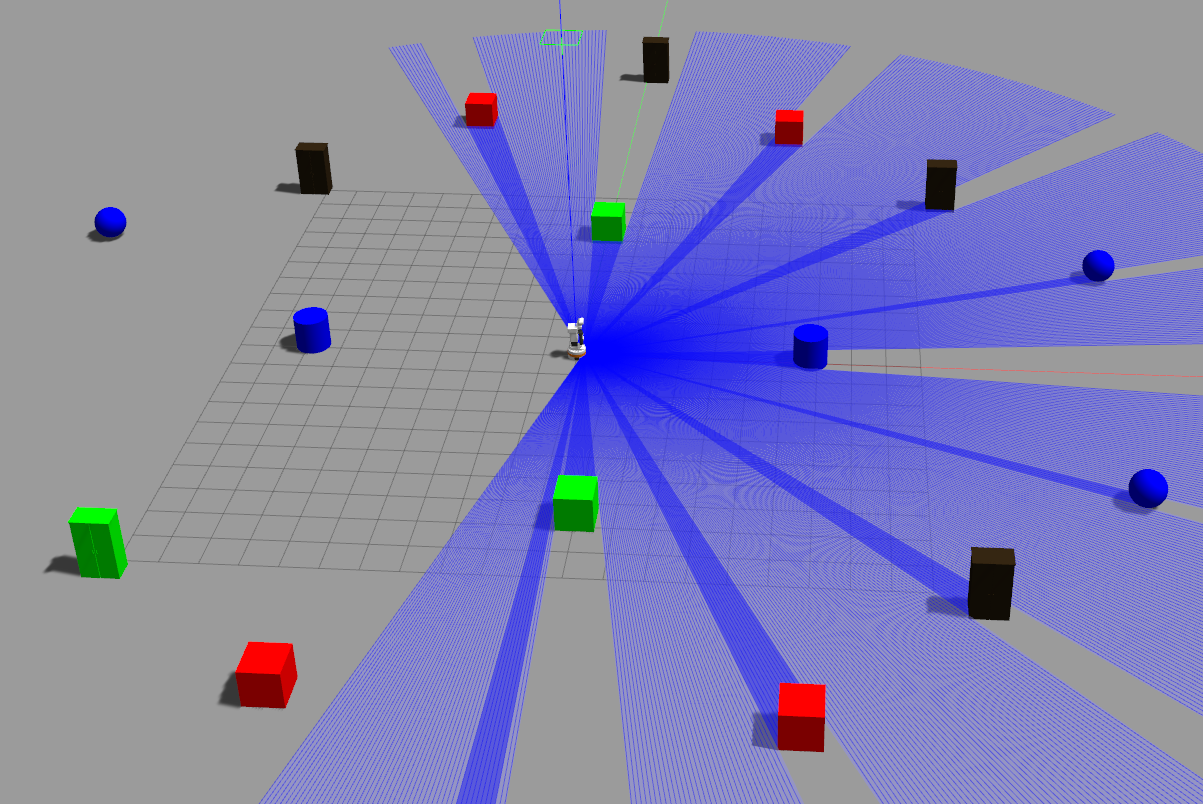
\includegraphics[width=1\textwidth]{Bilder/env3.png} 
\caption[]{Environment used for Batch 1.}
\label{env3}
\end{figure}

The following subsections, will list the parameters and graphs used for each model created by the pipeline. The manual test results, as defined in Section 4.4.3 in the main paper, are summarized in \secref{summary_batch_1}.

\newpage

\subsubsection{Model 1\label{model_1} }
\begin{multicols}{2}
\textbf{Data acquisition}
\begin{itemize}
\setlength\itemsep{0.1em}
\item recorded bagfiles: 10
\item recorded images: 600
\item angle avoidance: 45
\item timeout limit: 20
\item recording distance: 3.5
\item safe passage diameter: 2
\end{itemize}

\textbf{Feature Extraction}
\begin{itemize}
\setlength\itemsep{0.1em}
\item Dataset name: dataset\_1.h5
\item  laser range: 233:437
\item  laser sections: 5
\item  laser count: 666
\item  selection range: 2
\item  target count: 31
\item  laser threshold: 1.8
\end{itemize}

\columnbreak

\textbf{Training Model}
\begin{itemize}
\setlength\itemsep{0.1em}
\item  Model name: model\_1.h5
\item  No. of epochs: 15
\item  Steps: 1000
\item  Batch Size: 64
\item  Learning Rate: 0.0002
\item  Ratio val vs training: 0.85
\end{itemize}

\textbf{Testing Model}
\begin{itemize}
\setlength\itemsep{0.1em}
\item Rounds: 100
\newline
\newline
\newline
\newline
\newline
\newline
\newline
\newline
%\newline
\end{itemize}
\end{multicols}

\begin{figure}[h]%[htbp]
\centering
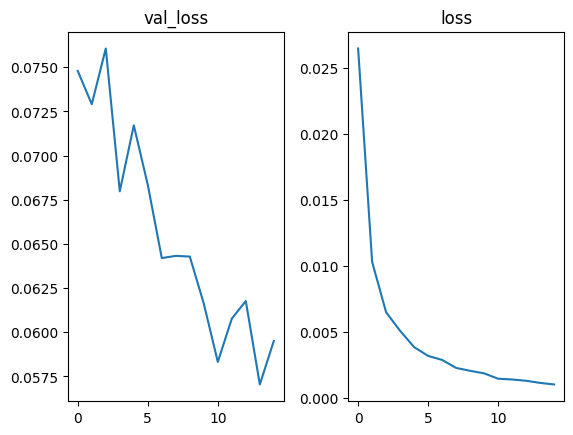
\includegraphics[width=8cm,height=6cm]{3_models/models_1/graph_1.png} 
\hspace{0.2 cm}
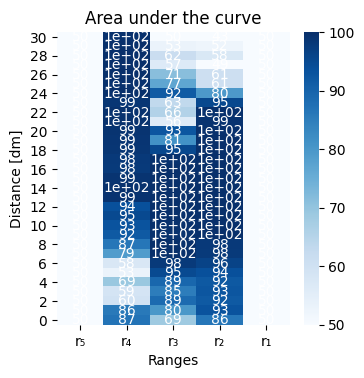
\includegraphics[width=6cm,height=6cm]{4_plots/plots_1/AUC_1.png} 
\caption[]{The left graph shows the validation versus the training loss while the right graph shows the summary of the Area under the Receiver operating characteristic Curve for all ranges from $\{r_{1}, ... ,r_{n}\}$ as well for all intermediary positions (distances).}
\label{theta_alt}
\end{figure}

\newpage


\subsubsection{Model 2\label{model_2} }
\begin{multicols}{2}
\textbf{Data acquisition}
\begin{itemize}
\setlength\itemsep{0.1em}
\item recorded bagfiles: 20
\item recorded images: 1200
\item angle avoidance: 45
\item timeout limit: 20
\item recording distance: 3.5
\item safe passage diameter: 2
\end{itemize}

\textbf{Feature Extraction}
\begin{itemize}
\setlength\itemsep{0.1em}
\item Dataset name: dataset\_2.h5
\item  laser range: 233:437
\item  laser sections: 5
\item  laser count: 666
\item  selection range: 2
\item  target count: 31
\item  laser threshold: 1.8
\end{itemize}

\columnbreak

\textbf{Training Model}
\begin{itemize}
\setlength\itemsep{0.1em}
\item  Model name: model\_2.h5
\item  No. of epochs: 15
\item  Steps: 1000
\item  Batch Size: 64
\item  Learning Rate: 0.0002
\item  Ratio val vs training: 0.85
\end{itemize}

\textbf{Testing Model}
\begin{itemize}
\setlength\itemsep{0.1em}
\item Rounds: 100
\newline
\newline
\newline
\newline
\newline
\newline
\newline
\newline
%\newline
\end{itemize}
\end{multicols}

\begin{figure}[h]%[htbp]
\centering
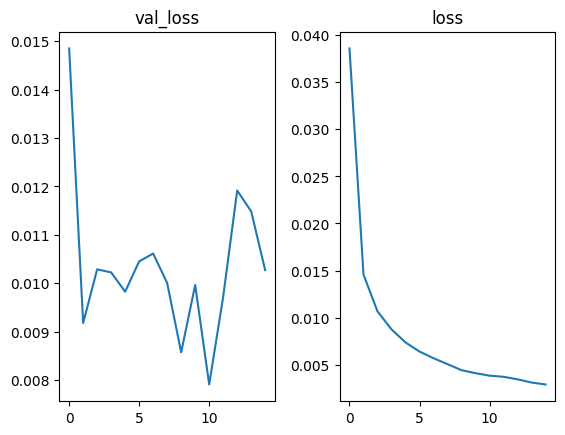
\includegraphics[width=8cm,height=6cm]{3_models/models_2/graph_2.png} 
\hspace{0.2 cm}
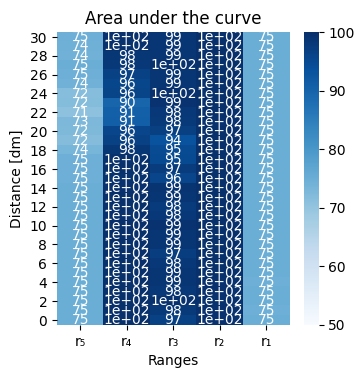
\includegraphics[width=6cm,height=6cm]{4_plots/plots_2/AUC_2.png} 
\caption[]{The left graph shows the validation versus the training loss while the right graph shows the summary of the Area Under the Receiver Operating Characteristic curve for all ranges from $\{r_{1}, ... ,r_{n}\}$ as well for all intermediary positions (distances).}
\label{theta_alt}
\end{figure}

\newpage

\subsubsection{Model 3\label{model_3} }
\begin{multicols}{2}
\textbf{Data acquisition}
\begin{itemize}
\setlength\itemsep{0.1em}
\item recorded bagfiles: 40
\item recorded images: 2400
\item angle avoidance: 45
\item timeout limit: 20
\item recording distance: 3.5
\item safe passage diameter: 2
\end{itemize}

\textbf{Feature Extraction}
\begin{itemize}
\setlength\itemsep{0.1em}
\item Dataset name: dataset\_3.h5
\item  laser range: 233:437
\item  laser sections: 5
\item  laser count: 666
\item  selection range: 2
\item  target count: 31
\item  laser threshold: 1.8
\end{itemize}

\columnbreak

\textbf{Training Model}
\begin{itemize}
\setlength\itemsep{0.1em}
\item  Model name: model\_3.h5
\item  No. of epochs: 15
\item  Steps: 1000
\item  Batch Size: 64
\item  Learning Rate: 0.0002
\item  Ratio val vs training: 0.85
\end{itemize}

\textbf{Testing Model}
\begin{itemize}
\setlength\itemsep{0.1em}
\item Rounds: 100
\newline
\newline
\newline
\newline
\newline
\newline
\newline
\newline
%\newline
\end{itemize}
\end{multicols}

\begin{figure}[h]%[htbp]
\centering
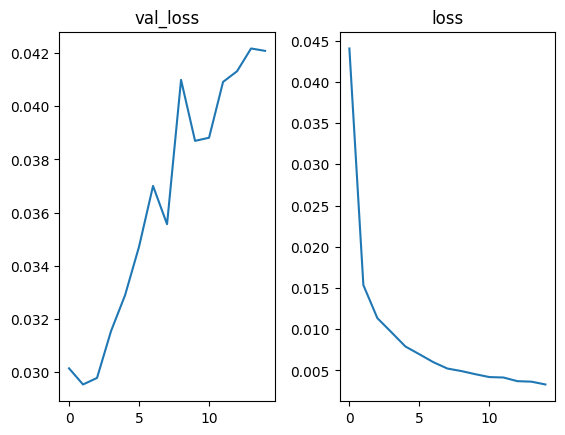
\includegraphics[width=8cm,height=6cm]{3_models/models_3/graph_3.png} 
\hspace{0.2 cm}
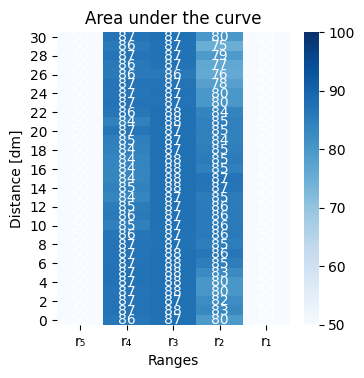
\includegraphics[width=6cm,height=6cm]{4_plots/plots_3/AUC_3.png} 
\caption[]{The left graph shows the validation versus the training loss while the right graph shows the summary of the Area under the Receiver operating characteristic Curve for all ranges from $\{r_{1}, ... ,r_{n}\}$ as well for all intermediary positions (distances).}
\label{theta_alt}
\end{figure}


\newpage
\subsubsection{Model 4\label{model_4} }
\begin{multicols}{2}\textbf{Data acquisition}
\begin{itemize}
\setlength\itemsep{0.1em}
\item recorded bagfiles: 80
\item recorded images: 4800
\item angle avoidance: 45
\item timeout limit: 20
\item recording distance: 3.5
\item safe passage diameter: 2
\end{itemize}
\textbf{Feature Extraction}
\begin{itemize}
\setlength\itemsep{0.1em}
\item Dataset name: dataset\_4.h5
\item  laser range: 233:437
\item  laser sections: 5
\item  laser count: 666
\item  selection range: 2
\item  target count: 31
\item  laser threshold: 1.8
\end{itemize}
\columnbreak\textbf{Training Model}
\begin{itemize}
\setlength\itemsep{0.1em}
\item  Model name: model\_4.h5
\item  No. of epochs: 2
\item  Steps: 10
\item  Batch Size: 64
\item  Learning Rate: 0.0002
\item  Ratio val vs training: 0.85
\end{itemize}
\textbf{Testing Model}
\begin{itemize}
\setlength\itemsep{0.1em}
\item Rounds: 100
\newline
\newline
\newline
\newline
\newline
\newline
\newline
\newline
\end{itemize}
\end{multicols}\begin{figure}[H]%[htbp]
\centering
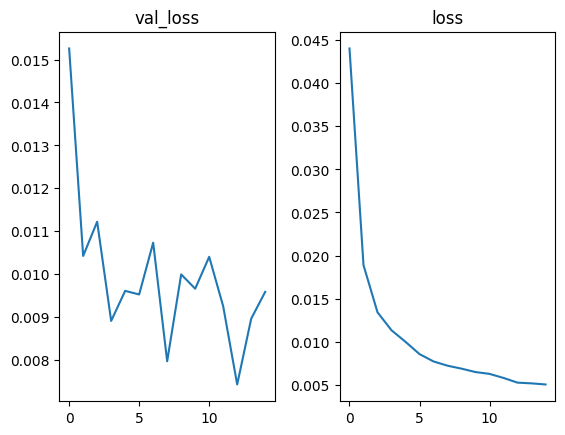
\includegraphics[width=8cm,height=6cm]{3_models/models_4/graph_4.png}
\hspace{0.2 cm}
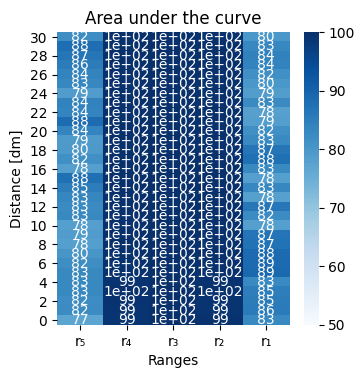
\includegraphics[width=6cm,height=6cm]{4_plots/plots_4/AUC_4.png}
\caption{The left graph shows the validation versus the training loss while the right graph shows the summary of the Area Under the Receiver Operating Characteristic curve for all ranges from $\{r_{1}, ... ,r_{n}\}$ as well for all intermediary positions (distances).}
\label{auc_7}
\end{figure}

\newpage
\subsubsection{Model 5\label{model_5} }
\begin{multicols}{2}\textbf{Data acquisition}
\begin{itemize}
\setlength\itemsep{0.1em}
\item recorded bagfiles: 160
\item recorded images: 9600
\item angle avoidance: 45
\item timeout limit: 20
\item recording distance: 3.5
\item safe passage diameter: 2
\end{itemize}
\textbf{Feature Extraction}
\begin{itemize}
\setlength\itemsep{0.1em}
\item Dataset name: dataset\_5.h5
\item  laser range: 233:437
\item  laser sections: 5
\item  laser count: 666
\item  selection range: 2
\item  target count: 31
\item  laser threshold: 1.8
\end{itemize}
\columnbreak\textbf{Training Model}
\begin{itemize}
\setlength\itemsep{0.1em}
\item  Model name: model\_5.h5
\item  No. of epochs: 2
\item  Steps: 10
\item  Batch Size: 64
\item  Learning Rate: 0.0002
\item  Ratio val vs training: 0.85
\end{itemize}
\textbf{Testing Model}
\begin{itemize}
\setlength\itemsep{0.1em}
\item Rounds: 100
\newline
\newline
\newline
\newline
\newline
\newline
\newline
\newline
\end{itemize}
\end{multicols}\begin{figure}[H]%[htbp]
\centering
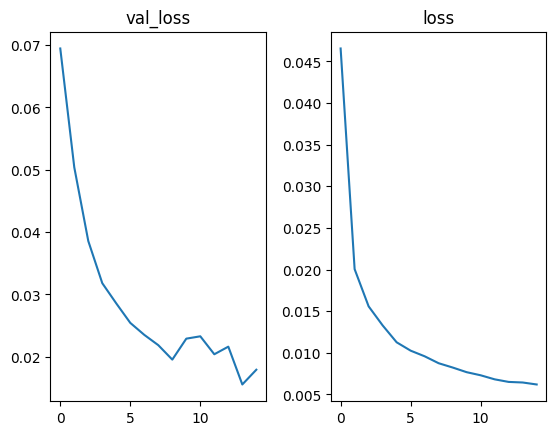
\includegraphics[width=8cm,height=6cm]{3_models/models_5/graph_5.png}
\hspace{0.2 cm}
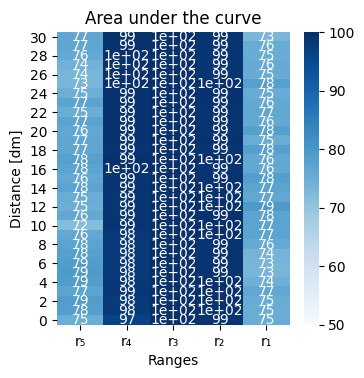
\includegraphics[width=6cm,height=6cm]{4_plots/plots_5/AUC_5.png}
\caption{The left graph shows the validation versus the training loss while the right graph shows the summary of the Area Under the Receiver Operating Characteristic curve for all ranges from $\{r_{1}, ... ,r_{n}\}$ as well for all intermediary positions (distances).}
\label{auc_7}
\end{figure}

\newpage
\subsubsection{Model 13\label{model_13} }
\begin{multicols}{2}\textbf{Data acquisition}
\begin{itemize}
\setlength\itemsep{0.1em}
\item recorded bagfiles: 320
\item recorded images: 19200
\item angle avoidance: 45
\item timeout limit: 20
\item recording distance: 3.0
\item safe passage diameter: 2
\end{itemize}
\textbf{Feature Extraction}
\begin{itemize}
\setlength\itemsep{0.1em}
\item Dataset name: dataset\_13.h5
\item  laser range: 233:437
\item  laser sections: 5
\item  laser count: 666
\item  selection range: 2
\item  target count: 31
\item  laser threshold: 1.8
\end{itemize}
\columnbreak\textbf{Training Model}
\begin{itemize}
\setlength\itemsep{0.1em}
\item  Model name: model\_13.h5
\item  No. of epochs: 15
\item  Steps: 1000
\item  Batch Size: 64
\item  Learning Rate: 0.0002
\item  Ratio val vs training: 0.85
\end{itemize}
\textbf{Testing Model}
\begin{itemize}
\setlength\itemsep{0.1em}
\item Rounds: 100
\newline
\newline
\newline
\newline
\newline
\newline
\newline
\newline
\end{itemize}
\end{multicols}\begin{figure}[H]%[htbp]
\centering
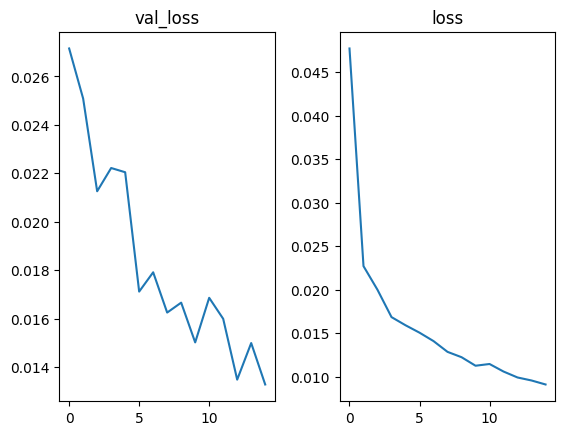
\includegraphics[width=8cm,height=6cm]{3_models/models_13/graph_13.png}
\hspace{0.2 cm}
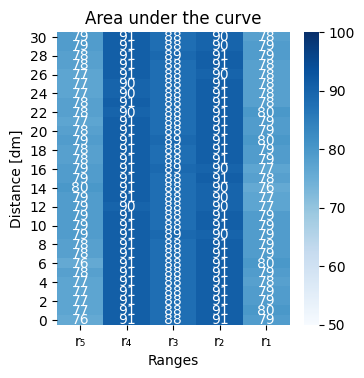
\includegraphics[width=6cm,height=6cm]{4_plots/plots_13/AUC_13.png}
\caption{The left graph shows the validation versus the training loss while the right graph shows the summary of the Area Under the Receiver Operating Characteristic curve for all ranges from $\{r_{1}, ... ,r_{n}\}$ as well for all intermediary positions (distances).}
\label{auc_13}
\end{figure}


\newpage
\subsubsection{Model 14\label{model_14} }
\begin{multicols}{2}\textbf{Data acquisition}
\begin{itemize}
\setlength\itemsep{0.1em}
\item recorded bagfiles: 320
\item recorded images: 19200
\item angle avoidance: 45
\item timeout limit: 20
\item recording distance: 3.0
\item safe passage diameter: 2
\end{itemize}
\textbf{Feature Extraction}
\begin{itemize}
\setlength\itemsep{0.1em}
\item Dataset name: dataset\_13.h5
\item  laser range: 233:437
\item  laser sections: 5
\item  laser count: 666
\item  selection range: 2
\item  target count: 31
\item  laser threshold: 1.8
\end{itemize}
\textbf{Training Model}
\begin{itemize}
\setlength\itemsep{0.1em}
\item  Model name: model\_14.h5
\item  No. of epochs: 15
\item  Steps: 1000
\item  Batch Size: 64
\item  Learning Rate: 0.002
\item  Ratio val vs training: 0.85
\end{itemize}
\textbf{Testing Model}
\begin{itemize}
\setlength\itemsep{0.1em}
\item Rounds: 100
\newline
\newline
\newline
\newline
\newline
\newline
\newline
\newline
\end{itemize}
\end{multicols}\begin{figure}[H]%[htbp]
\centering
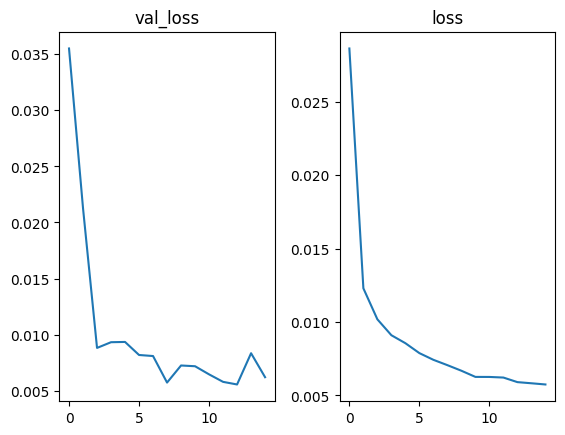
\includegraphics[width=8cm,height=6cm]{3_models/models_14/graph_14.png}
\hspace{0.2 cm}
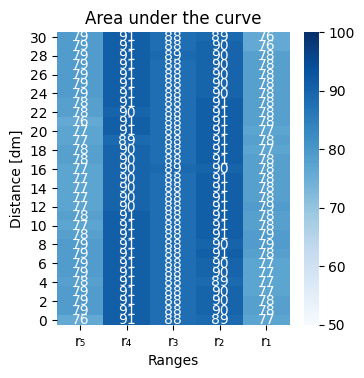
\includegraphics[width=6cm,height=6cm]{4_plots/plots_14/AUC_14.png}
\caption{The left graph shows the validation versus the training loss while the right graph shows the summary of the Area Under the Receiver Operating Characteristic curve for all ranges from $\{r_{1}, ... ,r_{n}\}$ as well for all intermediary positions (distances).}
\label{auc_14}
\end{figure}

\newpage
\subsubsection{Model 15\label{model_15} }
\begin{multicols}{2}\textbf{Data acquisition}
\begin{itemize}
\setlength\itemsep{0.1em}
\item recorded bagfiles: 320
\item recorded images: 19200
\item angle avoidance: 45
\item timeout limit: 20
\item recording distance: 3.0
\item safe passage diameter: 2
\end{itemize}
\textbf{Feature Extraction}
\begin{itemize}
\setlength\itemsep{0.1em}
\item Dataset name: dataset\_13.h5
\item  laser range: 233:437
\item  laser sections: 5
\item  laser count: 666
\item  selection range: 2
\item  target count: 31
\item  laser threshold: 1.8
\end{itemize}
\textbf{Training Model}
\begin{itemize}
\setlength\itemsep{0.1em}
\item  Model name: model\_15.h5
\item  No. of epochs: 15
\item  Steps: 1000
\item  Batch Size: 64
\item  Learning Rate: 0.02
\item  Ratio val vs training: 0.85
\end{itemize}
\textbf{Testing Model}
\begin{itemize}
\setlength\itemsep{0.1em}
\item Rounds: 100
\newline
\newline
\newline
\newline
\newline
\newline
\newline
\newline
\end{itemize}
\end{multicols}\begin{figure}[H]%[htbp]
\centering
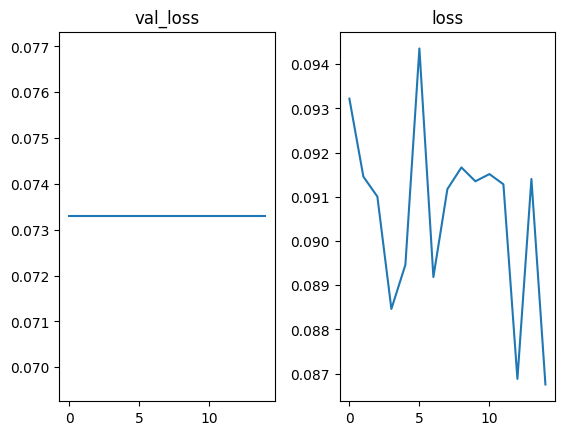
\includegraphics[width=8cm,height=6cm]{3_models/models_15/graph_15.png}
\hspace{0.2 cm}
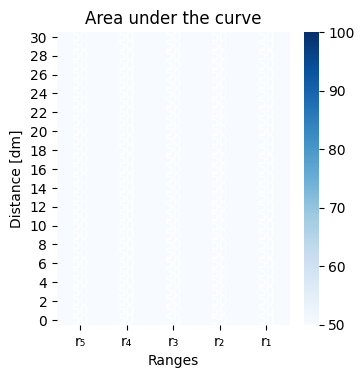
\includegraphics[width=6cm,height=6cm]{4_plots/plots_15/AUC_15.png}
\caption{The left graph shows the validation versus the training loss while the right graph shows the summary of the Area Under the Receiver Operating Characteristic curve for all ranges from $\{r_{1}, ... ,r_{n}\}$ as well for all intermediary positions (distances).}
\label{auc_15}
\end{figure}


\subsubsection{Summary\label{summary_batch_1} }
Table \ref{tab:summary_table_1} displays the summary of this batch. The tests are defined in Section 4.4.3 in the main paper. The table contains following information:
\begin{itemize}
\item  \textbf{Laser ranges: }Lowest to highest AUC result defined for each range
\item  \textbf{Unknown obstacles: }Performance result on unknown obstacles as two elements. The first element defines whether the model is able to properly recognize distances, while the second value, represents if ranges are predicted accurately.
\item  \textbf{Correct Distances: }Performance result for distances containing three elements. Each element represents a range of 1 meter starting with the first element from 0m to 1m with all subsequent elements alike.
\item  \textbf{Empty instances: }Result whether empty instance are recognized or not
\item  \textbf{Correct range: }Performance result for correct ranges to be recognized
\item  \textbf{Images recorded: }Amount of images recorded
\end{itemize}


% Please add the following required packages to your document preamble:
% \usepackage[table,xcdraw]{xcolor}
% If you use beamer only pass "xcolor=table" option, i.e. \documentclass[xcolor=table]{beamer}
\begin{table}[H]
\resizebox{\columnwidth}{!}{
\begin{tabular}{|c|c|c|c|c|c|c|c|c|c|c|c|}
\hline
\rowcolor[HTML]{020B36} 
{\color[HTML]{FFFFFF} \textbf{\begin{tabular}[c]{@{}c@{}}Model\\ name\end{tabular}}} & {\color[HTML]{FFFFFF} \textbf{$r_{5}$}} & {\color[HTML]{FFFFFF} \textbf{$r_{4}$}} & {\color[HTML]{FFFFFF} \textbf{$r_{3}$}} & {\color[HTML]{FFFFFF} \textbf{$r_{2}$}} & {\color[HTML]{FFFFFF} \textbf{$r_{1}$}} & {\color[HTML]{FFFFFF} \textbf{\begin{tabular}[c]{@{}c@{}}Learning\\ rate\end{tabular}}} & {\color[HTML]{FFFFFF} \textbf{\begin{tabular}[c]{@{}c@{}}Unknown\\ obstacles\end{tabular}}} & {\color[HTML]{FFFFFF} \textbf{\begin{tabular}[c]{@{}c@{}}Correct\\ distances\end{tabular}}} & {\color[HTML]{FFFFFF} \textbf{\begin{tabular}[c]{@{}c@{}}Empty\\ instances\end{tabular}}} & {\color[HTML]{FFFFFF} \textbf{\begin{tabular}[c]{@{}c@{}}Correct\\ range\end{tabular}}} & {\color[HTML]{FFFFFF} \textbf{\begin{tabular}[c]{@{}c@{}}Images\\ recorded\end{tabular}}} \\ \hline
\rowcolor[HTML]{FFFFFF} 
$M_{1}$                                                                              & 50 - 50                                 & 53 - 100                                & 50 - 100                                & 43 - 100                                & 50 - 50                                 & .0002                                                                                   & {[}0,0{]}                                                                                   & {[}0,0,.5{]}                                                                                & yes                                                                                       & {[}0,0,1,0,0{]}                                                                         & 600                                                                                       \\ \hline
\rowcolor[HTML]{FFFFFF} 
$M_{2}$                                                                              & 74 - 75                                 & 91 - 100                                & 94 -100                                 & 100 - 100                               & 75 - 75                                 & .0002                                                                                   & {[}0,0                                                                                      & {[}0,0,.5{]}                                                                                & yes                                                                                       & {[}0,0,0,0,0{]}                                                                         & 1200                                                                                      \\ \hline
\rowcolor[HTML]{FFFFFF} 
$M_{3}$                                                                              & 50 - 50                                 & 84 - 87                                 & 74 - 75                                 & 79 - 87                                 & 50 - 50                                 & .0002                                                                                   & {[}0,1{]}                                                                                   & {[}0,0,0{]}                                                                                 & yes                                                                                       & {[}.5,.5,.5,.5,.5{]}                                                                    & 2400                                                                                      \\ \hline
\rowcolor[HTML]{FFFFFF} 
$M_{4}$                                                                              & 77 - 87                                 & 99 - 100                                & 90 - 96                                 & 99 - 100                                & 78 - 89                                 & .0002                                                                                   & {[}0,1{]}                                                                                   & {[}0,0,0{]}                                                                                 & yes                                                                                       & {[}.5,.5,.1,.5,.5{]}                                                                    & 4800                                                                                      \\ \hline
\rowcolor[HTML]{FFFFFF} 
$M_{5}$                                                                              & 73 - 79                                 & 99 - 100                                & 75 - 84                                 & 99 - 100                                & 74 - 79                                 & .0002                                                                                   & {[}0,1{]}                                                                                   & {[}0,0,.8{]}                                                                                & yes                                                                                       & {[}1,1,1,1,1{]}                                                                         & 9600                                                                                      \\ \hline
\rowcolor[HTML]{FFFFFF} 
$M_{13}$                                                                             & 76 - 79                                 & 90 - 91                                 & 88 - 89                                 & 90 - 91                                 & 77 - 80                                 & .0002                                                                                   & {[}0,1{]}                                                                                   & {[}0,0,8{]}                                                                                 & yes                                                                                       & {[}0,1,1,1,0{]}                                                                         & 19200                                                                                     \\ \hline
\rowcolor[HTML]{FFFFFF} 
$M_{14}$                                                                             & 77 - 79                                 & 89 - 91                                 & 88 - 89                                 & 89 - 91                                 & 76 - 78                                 & .002                                                                                    & {[}0,0{]}                                                                                   & {[}0,0,8{]}                                                                                 & yes                                                                                       & {[}0,1,1,1,0{]}                                                                         & 19200                                                                                     \\ \hline
\rowcolor[HTML]{FFFFFF} 
$M_{15}$                                                                             & 50 - 50                                 & 50 - 50                                 & 50 - 50                                 & 50 - 50                                 & 50 - 50                                 & .02                                                                                     & {[}0,0{]}                                                                                   & {[}0,0,0{]}                                                                                 & no                                                                                        & {[}0,0,0,0,0{]}                                                                         & 19200                                                                                     \\ \hline
\end{tabular}
}
\caption{Summary table}
\label{tab:summary_table_1}
\end{table}


\newpage

\subsection{Batch 2 \label{batch_2} }
These are the test results for the second training batch which consists of 6 different models with its input images increased from 600 to 30000. \figref{env_1_3} displays the environment used for this batch. For this batch, a higher different amount of obstacles to train with is used which intuitively suggests to result in a lower performance, as the same amount of images are used.

\begin{figure}[H]%[htbp]
\centering
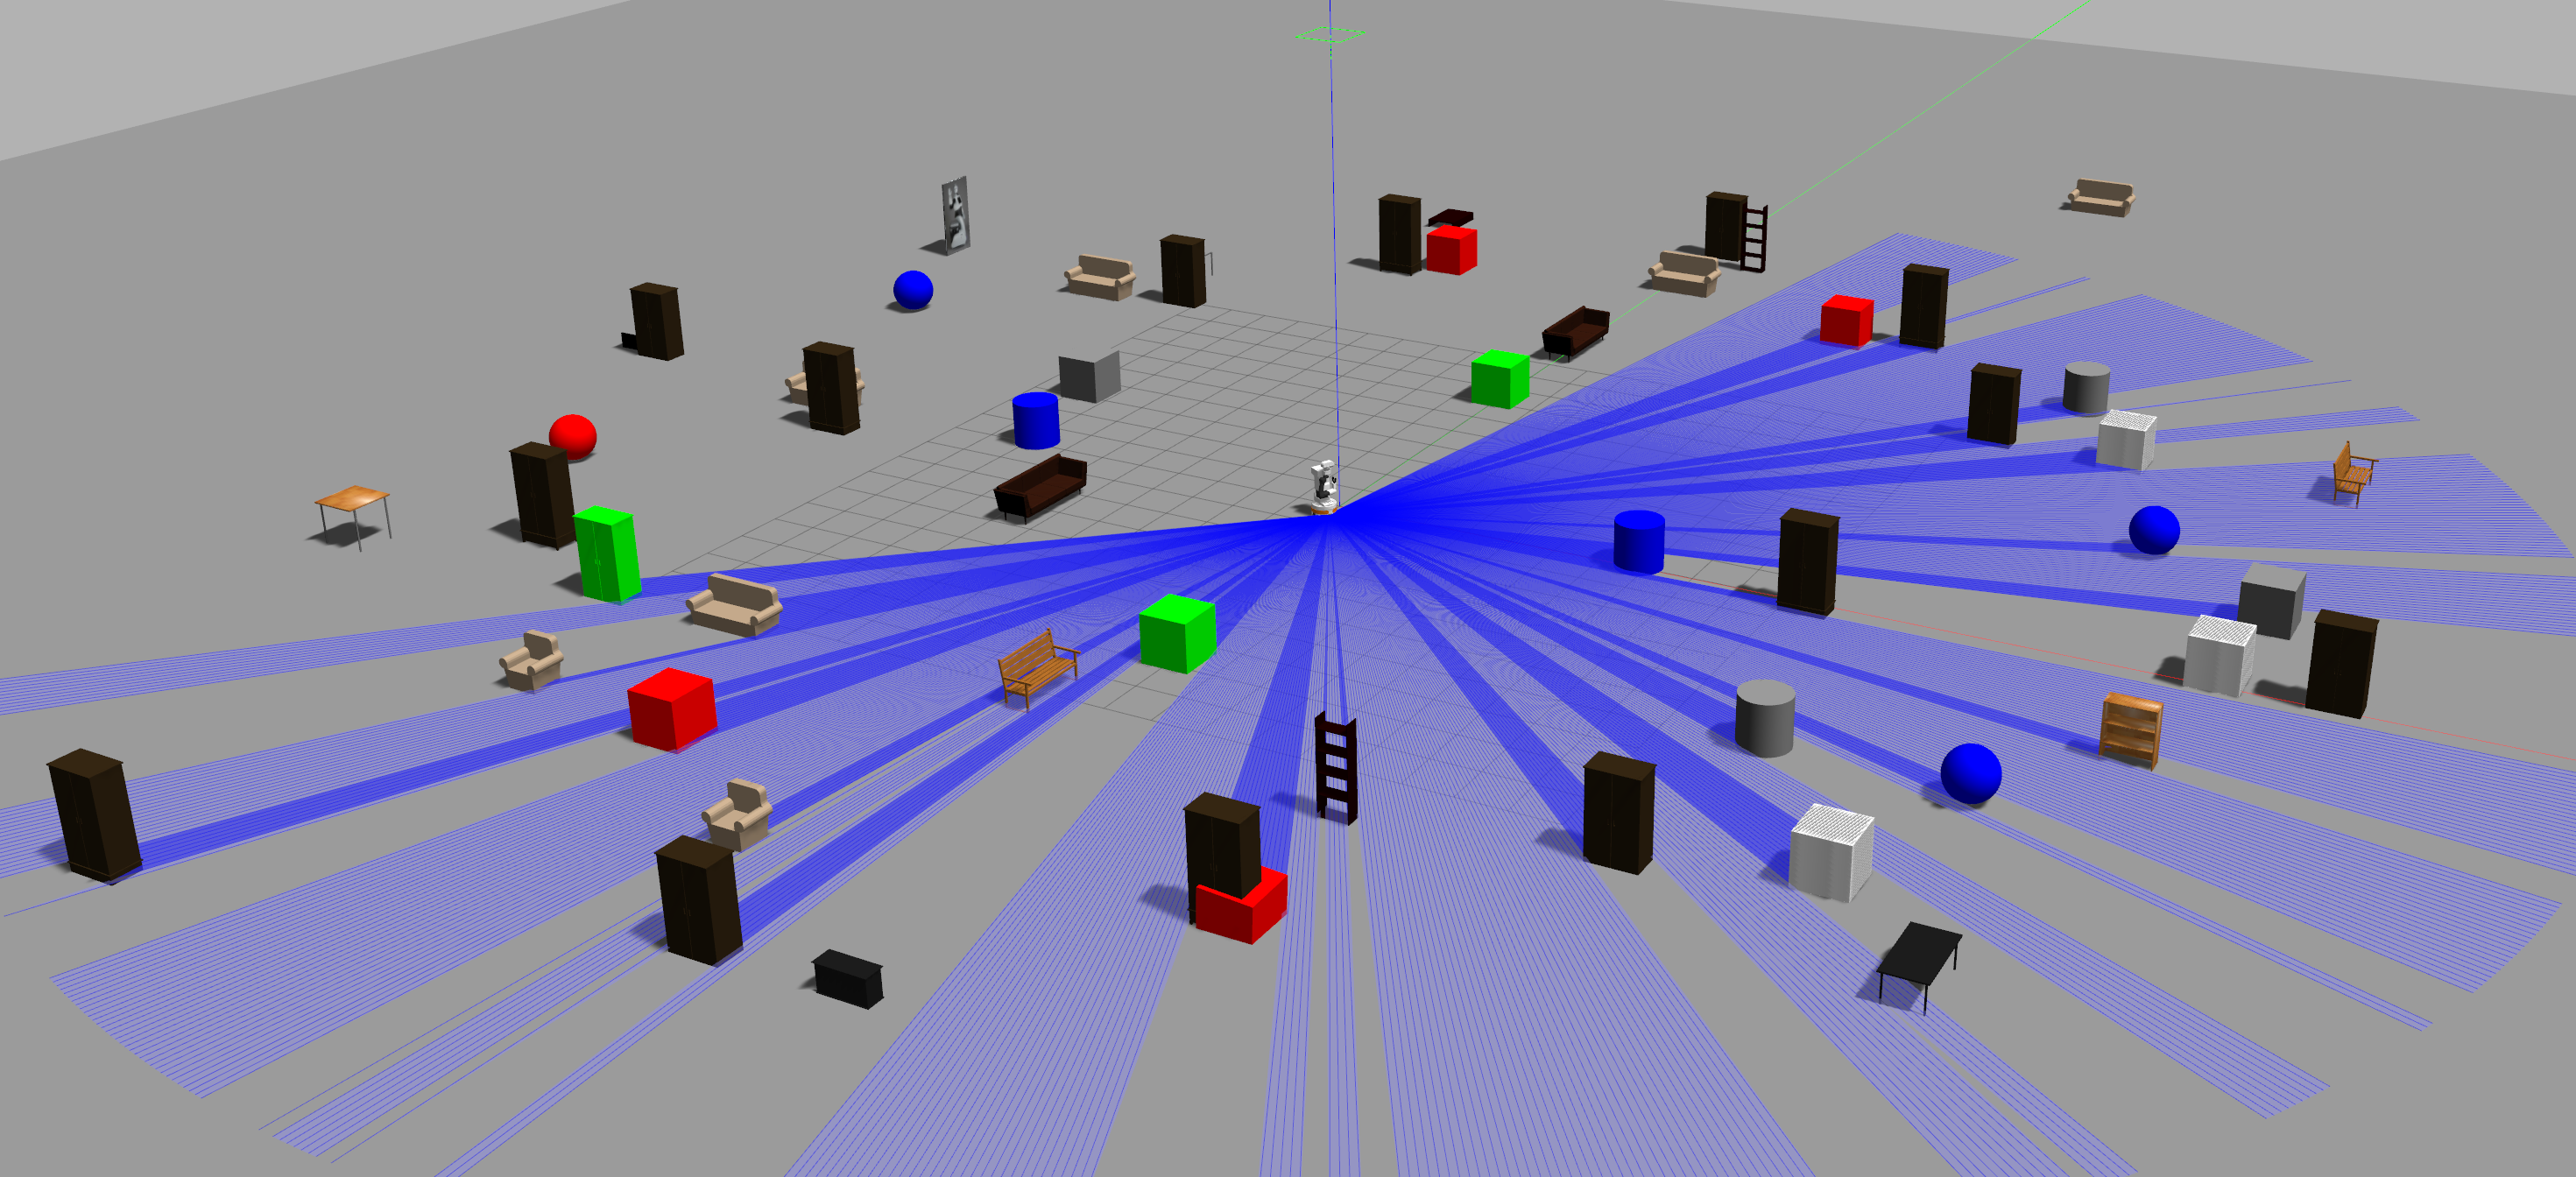
\includegraphics[width=1\textwidth]{Bilder/env1_env2_env3.png} 
\caption[]{Environment used for Batch 2.}
\label{env_1_3}
\end{figure}

\newpage
\subsubsection{Model 6\label{model_6} }
\begin{multicols}{2}\textbf{Data acquisition}
\begin{itemize}
\setlength\itemsep{0.1em}
\item recorded bagfiles: 10
\item recorded images: 600
\item angle avoidance: 45
\item timeout limit: 20
\item recording distance: 3.0
\item safe passage diameter: 2
\end{itemize}
\textbf{Feature Extraction}
\begin{itemize}
\setlength\itemsep{0.1em}
\item Dataset name: dataset\_6.h5
\item  laser range: 233:437
\item  laser sections: 5
\item  laser count: 666
\item  selection range: 2
\item  target count: 31
\item  laser threshold: 1.8
\end{itemize}
\columnbreak\textbf{Training Model}
\begin{itemize}
\setlength\itemsep{0.1em}
\item  Model name: model\_6.h5
\item  No. of epochs: 15
\item  Steps: 1000
\item  Batch Size: 64
\item  Learning Rate: 0.0002
\item  Ratio val vs training: 0.85
\end{itemize}
\textbf{Testing Model}
\begin{itemize}
\setlength\itemsep{0.1em}
\item Rounds: 100
\newline
\newline
\newline
\newline
\newline
\newline
\newline
\newline
\end{itemize}
\end{multicols}\begin{figure}[H]%[htbp]
\centering
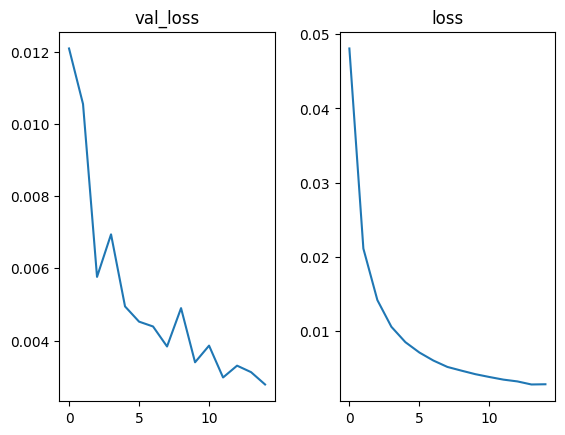
\includegraphics[width=8cm,height=6cm]{3_models/models_6/graph_6.png}
\hspace{0.2 cm}
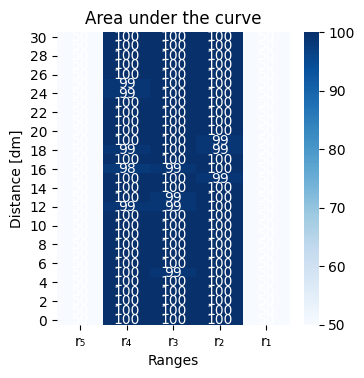
\includegraphics[width=6cm,height=6cm]{4_plots/plots_6/AUC_6.png}
\caption{The left graph shows the validation versus the training loss while the right graph shows the summary of the Area Under the Receiver Operating Characteristic curve for all ranges from $\{r_{1}, ... ,r_{n}\}$ as well for all intermediary positions (distances).}
\label{auc_6}
\end{figure}


\newpage
\subsubsection{Model 7\label{model_7} }
\begin{multicols}{2}\textbf{Data acquisition}
\begin{itemize}
\setlength\itemsep{0.1em}
\item recorded bagfiles: 20
\item recorded images: 1200
\item angle avoidance: 45
\item timeout limit: 20
\item recording distance: 3.0
\item safe passage diameter: 2
\end{itemize}
\textbf{Feature Extraction}
\begin{itemize}
\setlength\itemsep{0.1em}
\item Dataset name: dataset\_7.h5
\item  laser range: 233:437
\item  laser sections: 5
\item  laser count: 666
\item  selection range: 2
\item  target count: 31
\item  laser threshold: 1.8
\end{itemize}
\columnbreak\textbf{Training Model}
\begin{itemize}
\setlength\itemsep{0.1em}
\item  Model name: model\_7.h5
\item  No. of epochs: 15
\item  Steps: 1000
\item  Batch Size: 64
\item  Learning Rate: 0.0002
\item  Ratio val vs training: 0.85
\end{itemize}
\textbf{Testing Model}
\begin{itemize}
\setlength\itemsep{0.1em}
\item Rounds: 100
\newline
\newline
\newline
\newline
\newline
\newline
\newline
\newline
\end{itemize}
\end{multicols}\begin{figure}[H]%[htbp]
\centering
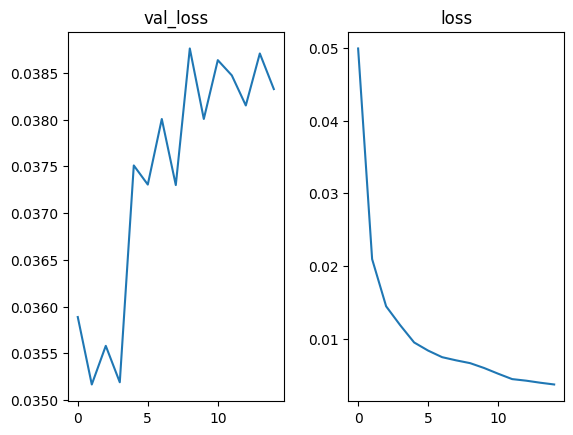
\includegraphics[width=8cm,height=6cm]{3_models/models_7/graph_7.png}
\hspace{0.2 cm}
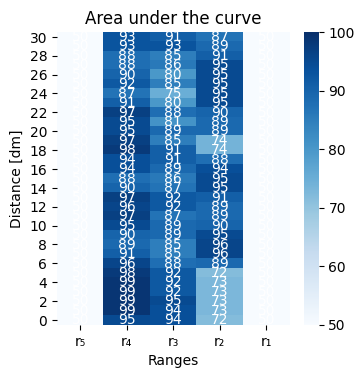
\includegraphics[width=6cm,height=6cm]{4_plots/plots_7/AUC_7.png}
\caption{The left graph shows the validation versus the training loss while the right graph shows the summary of the Area Under the Receiver Operating Characteristic curve for all ranges from $\{r_{1}, ... ,r_{n}\}$ as well for all intermediary positions (distances).}
\label{auc_7}
\end{figure}

\newpage
\subsubsection{Model 8\label{model_8} }
\begin{multicols}{2}\textbf{Data acquisition}
\begin{itemize}
\setlength\itemsep{0.1em}
\item recorded bagfiles: 40
\item recorded images: 2400
\item angle avoidance: 45
\item timeout limit: 20
\item recording distance: 3.0
\item safe passage diameter: 2
\end{itemize}
\textbf{Feature Extraction}
\begin{itemize}
\setlength\itemsep{0.1em}
\item Dataset name: dataset\_8.h5
\item  laser range: 233:437
\item  laser sections: 5
\item  laser count: 666
\item  selection range: 2
\item  target count: 31
\item  laser threshold: 1.8
\end{itemize}
\columnbreak\textbf{Training Model}
\begin{itemize}
\setlength\itemsep{0.1em}
\item  Model name: model\_8.h5
\item  No. of epochs: 15
\item  Steps: 1000
\item  Batch Size: 64
\item  Learning Rate: 0.0002
\item  Ratio val vs training: 0.85
\end{itemize}
\textbf{Testing Model}
\begin{itemize}
\setlength\itemsep{0.1em}
\item Rounds: 100
\newline
\newline
\newline
\newline
\newline
\newline
\newline
\newline
\end{itemize}
\end{multicols}\begin{figure}[H]%[htbp]
\centering
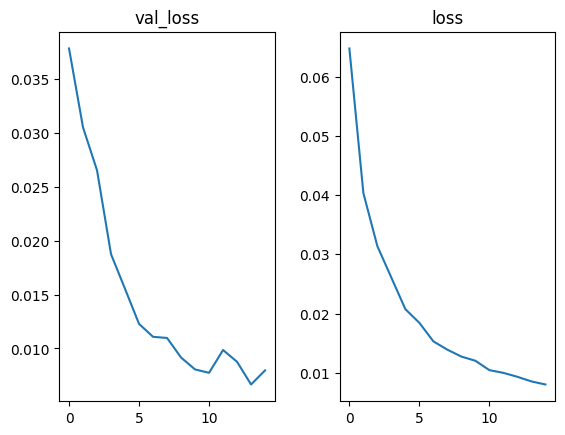
\includegraphics[width=8cm,height=6cm]{3_models/models_8/graph_8.png}
\hspace{0.2 cm}
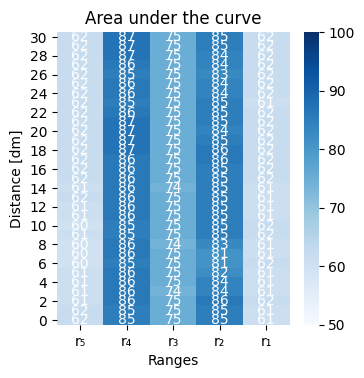
\includegraphics[width=6cm,height=6cm]{4_plots/plots_8/AUC_8.png}
\caption{The left graph shows the validation versus the training loss while the right graph shows the summary of the Area Under the Receiver Operating Characteristic curve for all ranges from $\{r_{1}, ... ,r_{n}\}$ as well for all intermediary positions (distances).}
\label{auc_8}
\end{figure}

\newpage
\subsubsection{Model 9\label{model_9} }
\begin{multicols}{2}\textbf{Data acquisition}
\begin{itemize}
\setlength\itemsep{0.1em}
\item recorded bagfiles: 80
\item recorded images: 4800
\item angle avoidance: 45
\item timeout limit: 20
\item recording distance: 3.0
\item safe passage diameter: 2
\end{itemize}
\textbf{Feature Extraction}
\begin{itemize}
\setlength\itemsep{0.1em}
\item Dataset name: dataset\_9.h5
\item  laser range: 233:437
\item  laser sections: 5
\item  laser count: 666
\item  selection range: 2
\item  target count: 31
\item  laser threshold: 1.8
\end{itemize}
\columnbreak\textbf{Training Model}
\begin{itemize}
\setlength\itemsep{0.1em}
\item  Model name: model\_9.h5
\item  No. of epochs: 15
\item  Steps: 1000
\item  Batch Size: 64
\item  Learning Rate: 0.0002
\item  Ratio val vs training: 0.85
\end{itemize}
\textbf{Testing Model}
\begin{itemize}
\setlength\itemsep{0.1em}
\item Rounds: 100
\newline
\newline
\newline
\newline
\newline
\newline
\newline
\newline
\end{itemize}
\end{multicols}\begin{figure}[H]%[htbp]
\centering
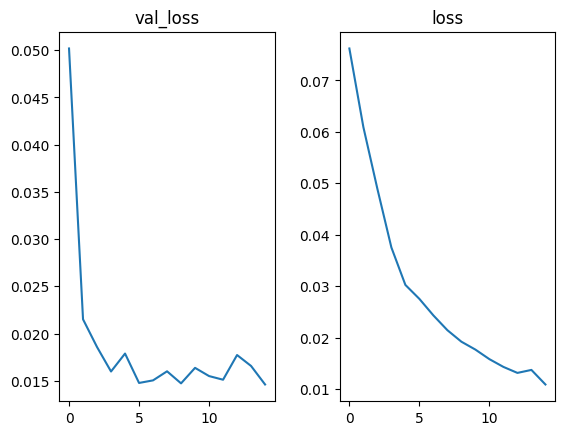
\includegraphics[width=8cm,height=6cm]{3_models/models_9/graph_9.png}
\hspace{0.2 cm}
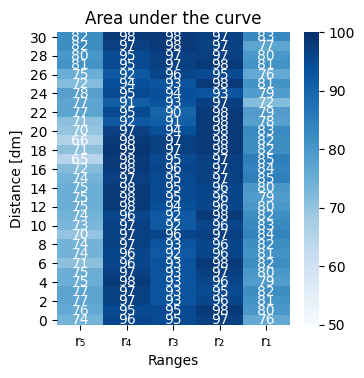
\includegraphics[width=6cm,height=6cm]{4_plots/plots_9/AUC_9.png}
\caption{The left graph shows the validation versus the training loss while the right graph shows the summary of the Area Under the Receiver Operating Characteristic curve for all ranges from $\{r_{1}, ... ,r_{n}\}$ as well for all intermediary positions (distances).}
\label{auc_9}
\end{figure}


\newpage
\subsubsection{Model 10\label{model_10} }
\begin{multicols}{2}\textbf{Data acquisition}
\begin{itemize}
\setlength\itemsep{0.1em}
\item recorded bagfiles: 160
\item recorded images: 9600
\item angle avoidance: 45
\item timeout limit: 20
\item recording distance: 3.0
\item safe passage diameter: 2
\end{itemize}
\textbf{Feature Extraction}
\begin{itemize}
\setlength\itemsep{0.1em}
\item Dataset name: dataset\_10.h5
\item  laser range: 233:437
\item  laser sections: 5
\item  laser count: 666
\item  selection range: 2
\item  target count: 31
\item  laser threshold: 1.8
\end{itemize}
\columnbreak\textbf{Training Model}
\begin{itemize}
\setlength\itemsep{0.1em}
\item  Model name: model\_10.h5
\item  No. of epochs: 15
\item  Steps: 1000
\item  Batch Size: 64
\item  Learning Rate: 0.0002
\item  Ratio val vs training: 0.85
\end{itemize}
\textbf{Testing Model}
\begin{itemize}
\setlength\itemsep{0.1em}
\item Rounds: 100
\newline
\newline
\newline
\newline
\newline
\newline
\newline
\newline
\end{itemize}
\end{multicols}\begin{figure}[H]%[htbp]
\centering
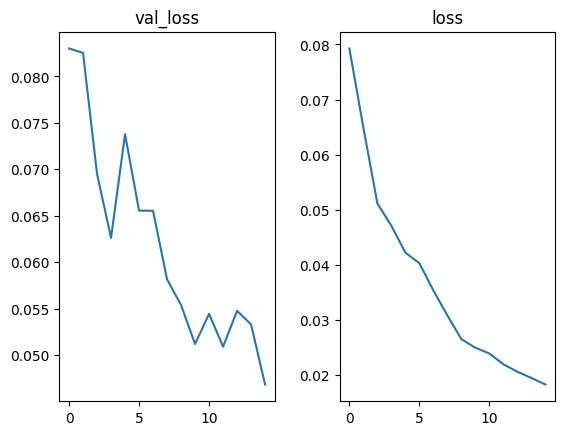
\includegraphics[width=8cm,height=6cm]{3_models/models_10/graph_10.png}
\hspace{0.2 cm}
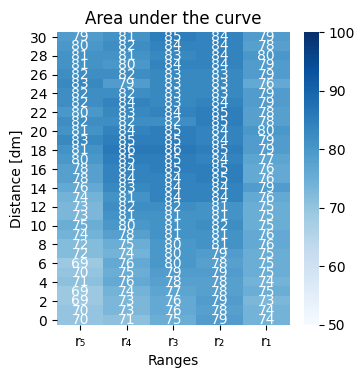
\includegraphics[width=6cm,height=6cm]{4_plots/plots_10/AUC_10.png}
\caption{The left graph shows the validation versus the training loss while the right graph shows the summary of the Area Under the Receiver Operating Characteristic curve for all ranges from $\{r_{1}, ... ,r_{n}\}$ as well for all intermediary positions (distances).}
\label{auc_10}
\end{figure}

\newpage
\subsubsection{Model 11\label{model_11} }
\begin{multicols}{2}\textbf{Data acquisition}
\begin{itemize}
\setlength\itemsep{0.1em}
\item recorded bagfiles: 500
\item recorded images: 30000
\end{itemize}
\textbf{Feature Extraction}
\begin{itemize}
\setlength\itemsep{0.1em}
\item Dataset name: dataset\_11.h5
\item  laser range: 233:437
\item  laser sections: 5
\item  laser count: 666
\item  selection range: 2
\item  target count: 31
\item  laser threshold: 1.8
\end{itemize}
\columnbreak\textbf{Training Model}
\begin{itemize}
\setlength\itemsep{0.1em}
\item  Model name: model\_11.h5
\item  No. of epochs: 15
\item  Steps: 1000
\item  Batch Size: 64
\item  Learning Rate: 0.0002
\item  Ratio val vs training: 0.85
\end{itemize}
\textbf{Testing Model}
\begin{itemize}
\setlength\itemsep{0.1em}
\item Rounds: 100
\newline
\newline
\newline
\newline
\newline
\newline
\newline
\newline
\end{itemize}
\end{multicols}\begin{figure}[H]%[htbp]
\centering
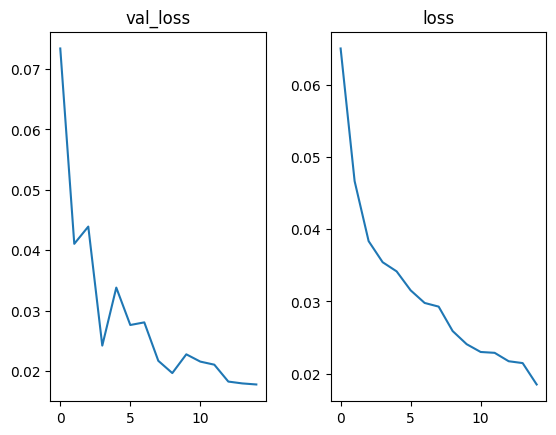
\includegraphics[width=8cm,height=6cm]{3_models/models_11/graph_11.png}
\hspace{0.2 cm}
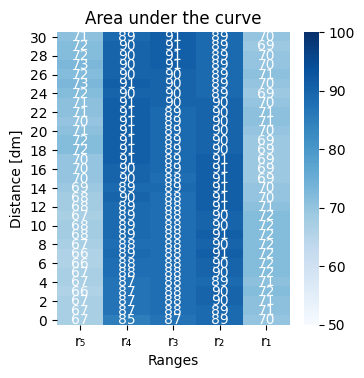
\includegraphics[width=6cm,height=6cm]{4_plots/plots_11/AUC_11.png}
\caption{The left graph shows the validation versus the training loss while the right graph shows the summary of the Area Under the Receiver Operating Characteristic curve for all ranges from $\{r_{1}, ... ,r_{n}\}$ as well for all intermediary positions (distances).}
\label{auc_11}
\end{figure}


\subsubsection{Summary\label{summary_batch_2} }
Table \ref{tab:summary_table_2} displays the summary of this batch. The tests are defined in Section 4.4.3 in the main paper. The table contains following information:
\begin{itemize}
\item  \textbf{Laser ranges: }Lowest to highest AUC result defined for each range
\item  \textbf{Unknown obstacles: }Performance result on unknown obstacles as two elements. The first element defines whether the model is able to properly recognize distances, while the second value, represents if ranges are predicted accurately.
\item  \textbf{Correct Distances: }Performance result for distances containing three elements. Each element represents a range of 1 meter starting with the first element from 0m to 1m with all subsequent elements alike.
\item  \textbf{Empty instances: }Result whether empty instance are recognized or not
\item  \textbf{Correct range: }Performance result for correct ranges to be recognized
\item  \textbf{Images recorded: }Amount of images recorded
\end{itemize}

%https://www.tablesgenerator.com/latex_tables/load
% Please add the following required packages to your document preamble:
% \usepackage[table,xcdraw]{xcolor}
% If you use beamer only pass "xcolor=table" option, i.e. \documentclass[xcolor=table]{beamer}
\begin{table}[H]
\resizebox{\columnwidth}{!}{%
\begin{tabular}{|c|c|c|c|c|c|c|c|c|c|c|c|}
\hline
\rowcolor[HTML]{020B36} 
{\color[HTML]{FFFFFF} \textbf{\begin{tabular}[c]{@{}c@{}}Model\\ name\end{tabular}}} & {\color[HTML]{FFFFFF} \textbf{$r_{5}$}} & {\color[HTML]{FFFFFF} \textbf{$r_{4}$}} & {\color[HTML]{FFFFFF} \textbf{$r_{3}$}} & {\color[HTML]{FFFFFF} \textbf{$r_{2}$}} & {\color[HTML]{FFFFFF} \textbf{$r_{1}$}} & {\color[HTML]{FFFFFF} \textbf{\begin{tabular}[c]{@{}c@{}}Learning\\ rate\end{tabular}}} & {\color[HTML]{FFFFFF} \textbf{\begin{tabular}[c]{@{}c@{}}Unknown\\ obstacles\end{tabular}}} & {\color[HTML]{FFFFFF} \textbf{\begin{tabular}[c]{@{}c@{}}Correct\\ Distance\end{tabular}}} & {\color[HTML]{FFFFFF} \textbf{\begin{tabular}[c]{@{}c@{}}Empty\\ instances\end{tabular}}} & {\color[HTML]{FFFFFF} \textbf{\begin{tabular}[c]{@{}c@{}}Correct\\ range\end{tabular}}} & {\color[HTML]{FFFFFF} \textbf{\begin{tabular}[c]{@{}c@{}}Images\\ recorded\end{tabular}}} \\ \hline
\rowcolor[HTML]{FFFFFF} 
$M_{6}$                                                                              & 50 - 50                                 & 98 - 100                                & 99 -100                                 & 99 - 100                                & 50 - 50                                 & .0002                                                                                   & {[}0,0{]}                                                                                   & {[}0,0,0{]}                                                                                & no                                                                                        & {[}0,0,0,0,0{]}                                                                         & 600                                                                                       \\ \hline
\rowcolor[HTML]{FFFFFF} 
$M_{7}$                                                                              & 50 - 50                                 & 88 - 98                                 & 80 - 94                                 & 72 - 96                                 & 50 - 50                                 & .0002                                                                                   & {[}0,.5{]}                                                                                  & {[}0,.5,.8{]}                                                                              & yes                                                                                       & {[}.6,.6,.6,.6,.6{]}                                                                    & 1200                                                                                      \\ \hline
\rowcolor[HTML]{FFFFFF} 
$M_{8}$                                                                              & 60 - 62                                 & 85 - 87                                 & 74 - 75                                 & 81 - 86                                 & 61 -62                                  & .0002                                                                                   & {[}0,.8{]}                                                                                  & {[}0,0,.8{]}                                                                               & yes                                                                                       & {[}.8,.8,.8,.8,.8{]}                                                                    & 2400                                                                                      \\ \hline
\rowcolor[HTML]{FFFFFF} 
$M_{9}$                                                                              & 65 - 81                                 & 91 - 99                                 & 90 - 96                                 & 93 - 98                                 & 76 -85                                  & .0002                                                                                   & {[}0,.9{]}                                                                                  & {[}0,0,.8{]}                                                                               & partially                                                                                 & {[}.7,.7,.7,.7,.7{]}                                                                    & 4800                                                                                      \\ \hline
\rowcolor[HTML]{FFFFFF} 
$M_{10}$                                                                             & 69 - 83                                 & 71 - 85                                 & 75 - 84                                 & 78 - 85                                 & 74 - 80                                 & .0002                                                                                   & {[}0,.9{]}                                                                                  & {[}0,0,.9{]}                                                                               & yes                                                                                       & {[}.9,.9,.9,.9,.9{]}                                                                    & 9600                                                                                      \\ \hline
\rowcolor[HTML]{FFFFFF} 
$M_{11}$                                                                             & 66 - 73                                 & 85 - 91                                 & 87 - 91                                 & 89 - 91                                 & 69 - 71                                 & .0002                                                                                   & {[}0,.9{]}                                                                                  & {[}0,0,.9{]}                                                                               & yes                                                                                       & {[}.9,.9,.9,.9,.9{]}                                                                    & 30000                                                                                     \\ \hline
\end{tabular}
}
\caption{Summary table}
\label{tab:summary_table_2}
\end{table}

\newpage

\subsection{Batch 3 \label{batch_3} }
These are the test results for the third training batch, which consists of 7 different models with the number of images increased from 600 to 9600. \figref{env4} displays the environment used for this batch.

\begin{figure}[H]%[htbp]
\centering
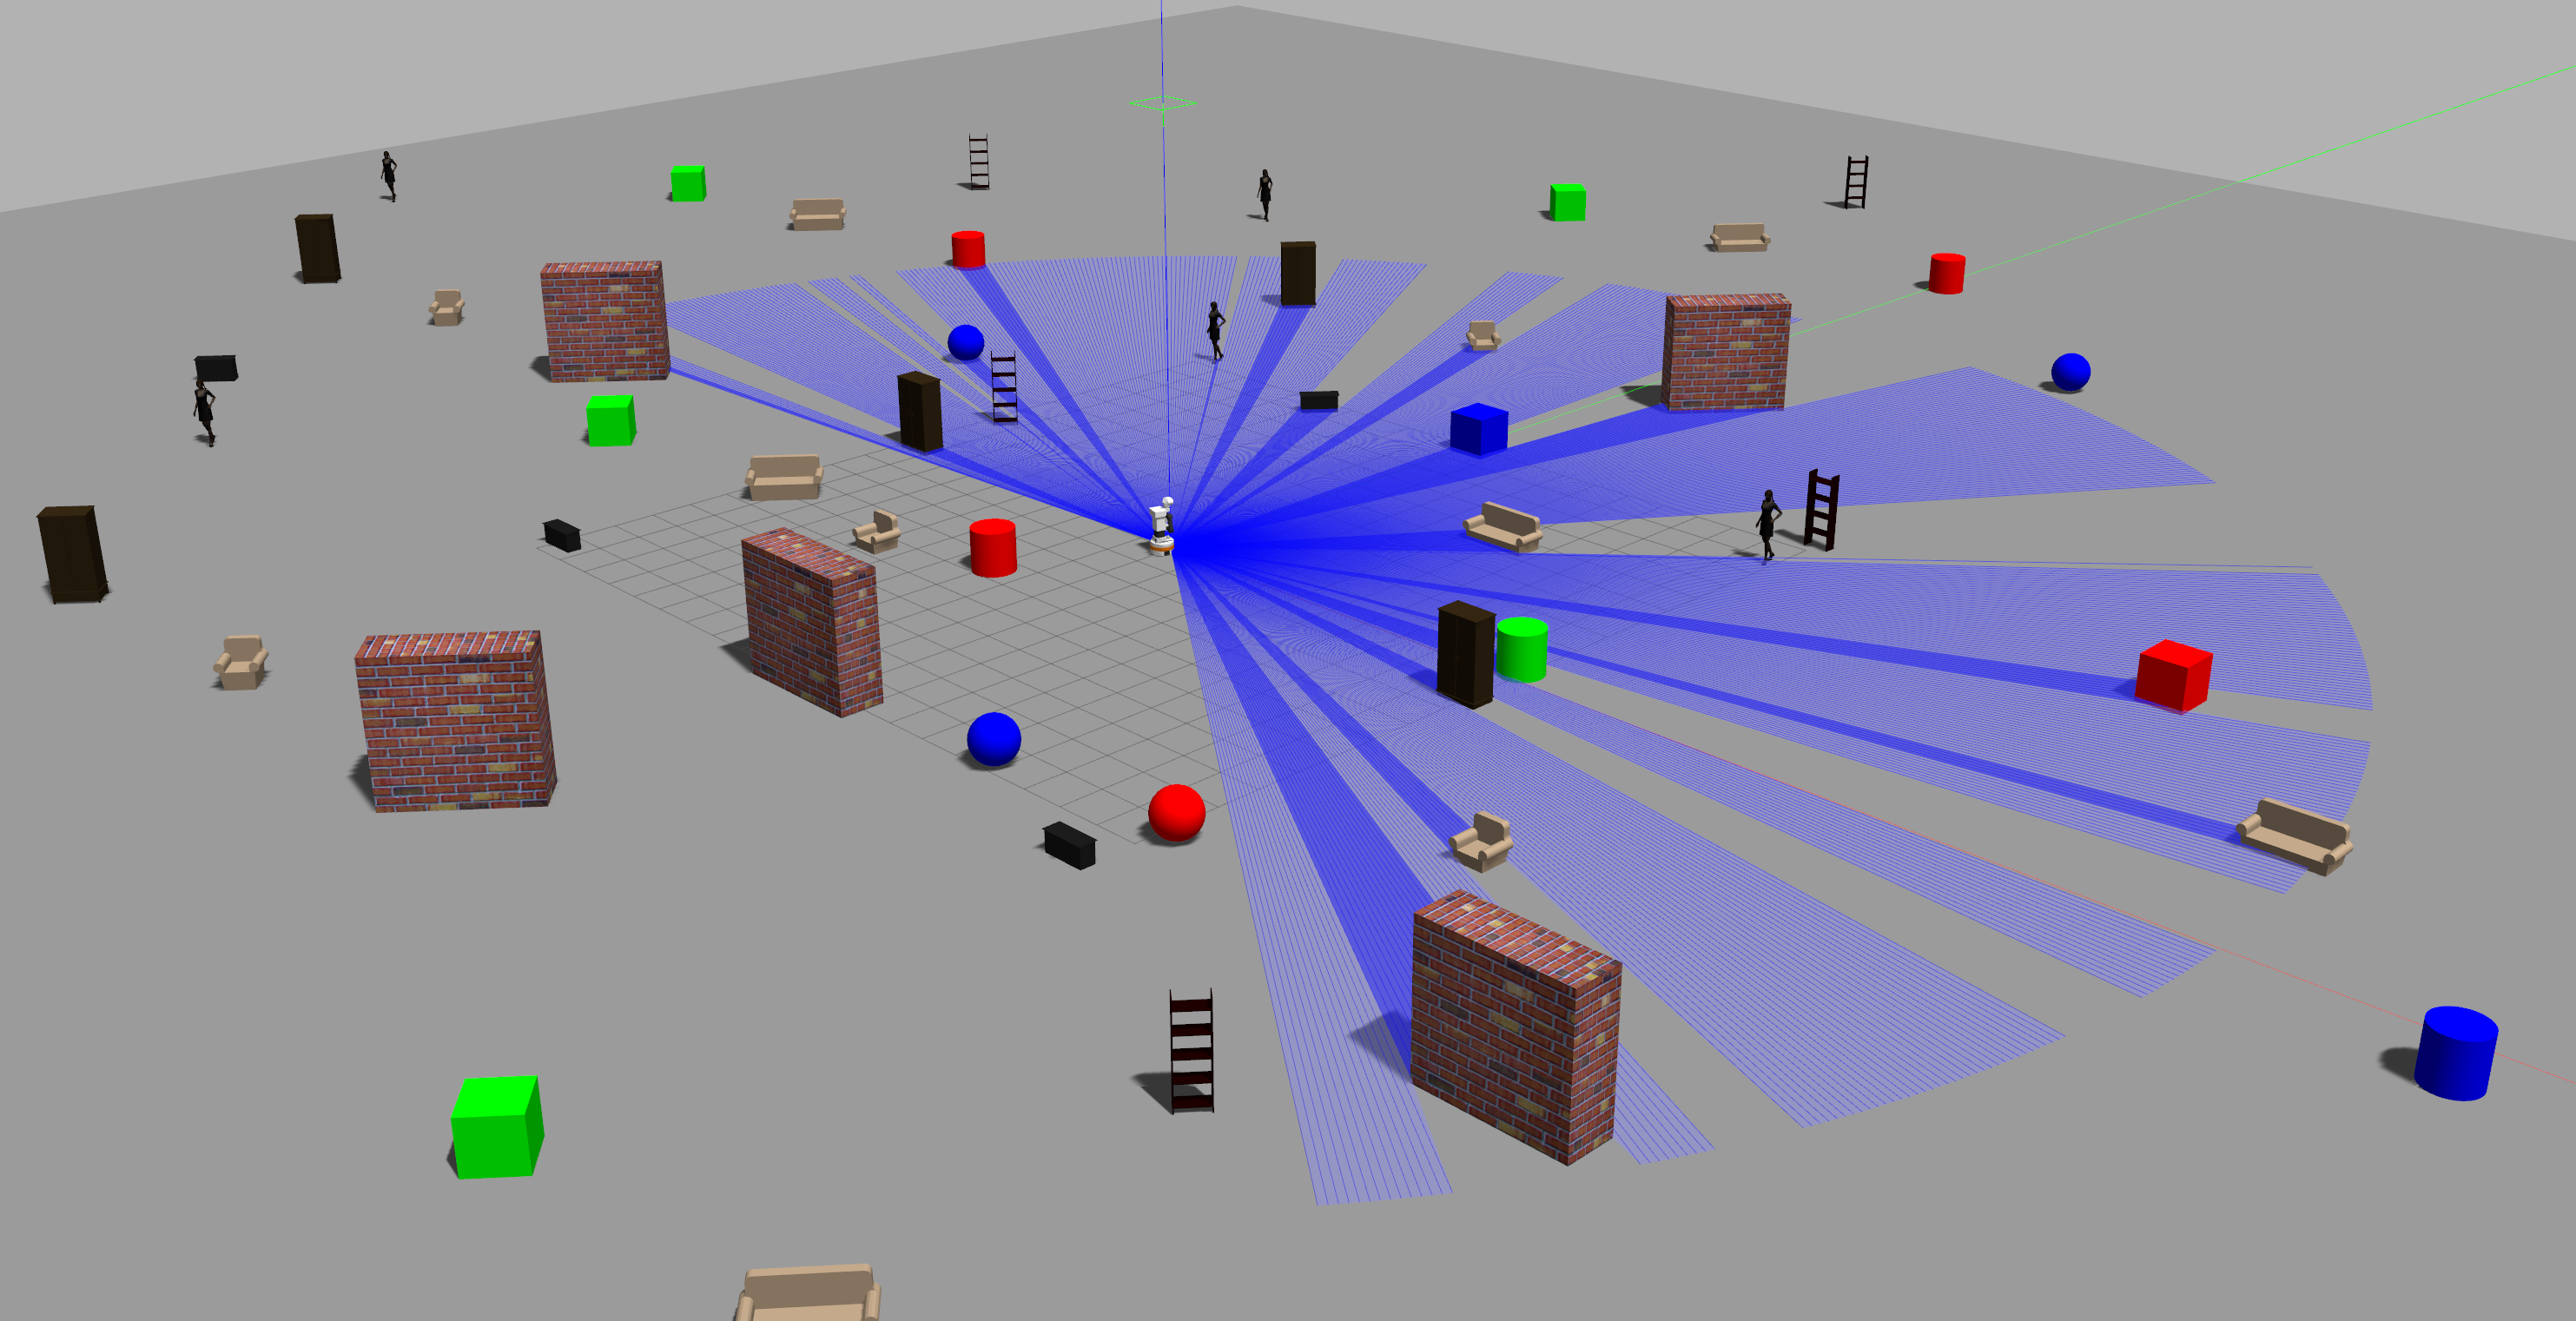
\includegraphics[width=1\textwidth]{Bilder/env4.png} 
\caption[]{Environment used for Batch 3.}
\label{env4}
\end{figure}

The following subsections, will list the parameters and graphs used for each model created by the pipeline. The manual test results, as defined in Section 4.4.3 in the main paper, are summarized in \secref{summary_batch_3}.

\newpage
\subsubsection{Model 17\label{model_17} }
\begin{multicols}{2}\textbf{Data acquisition}
\begin{itemize}
\setlength\itemsep{0.1em}
\item recorded bagfiles: 10
\item recorded images: 600
\item angle avoidance: 45
\item timeout limit: 20
\item recording distance: 3.0
\item safe passage diameter: 2
\end{itemize}
\textbf{Feature Extraction}
\begin{itemize}
\setlength\itemsep{0.1em}
\item Dataset name: dataset\_17.h5
\item  laser range: 233:437
\item  laser sections: 5
\item  laser count: 666
\item  selection range: 2
\item  target count: 31
\item  laser threshold: 0.8
\end{itemize}
\columnbreak\textbf{Training Model}
\begin{itemize}
\setlength\itemsep{0.1em}
\item  Model name: model\_17.h5
\item  No. of epochs: 15
\item  Steps: 1000
\item  Batch Size: 64
\item  Learning Rate: 0.0002
\item  Ratio val vs training: 0.85
\end{itemize}
\textbf{Testing Model}
\begin{itemize}
\setlength\itemsep{0.1em}
\item Rounds: 100
\newline
\newline
\newline
\newline
\newline
\newline
\newline
\newline
\end{itemize}
\end{multicols}\begin{figure}[H]%[htbp]
\centering
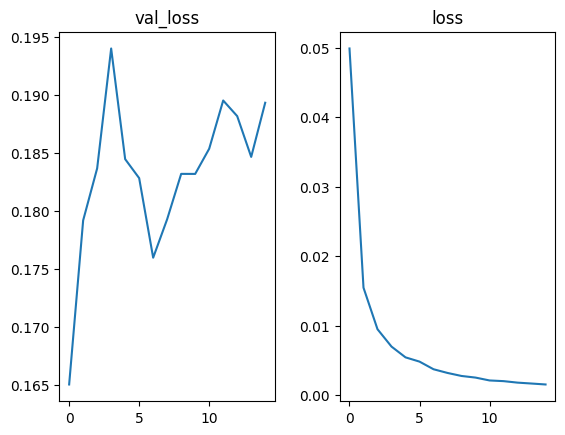
\includegraphics[width=8cm,height=6cm]{3_models/models_17/graph_17.png}
\hspace{0.2 cm}
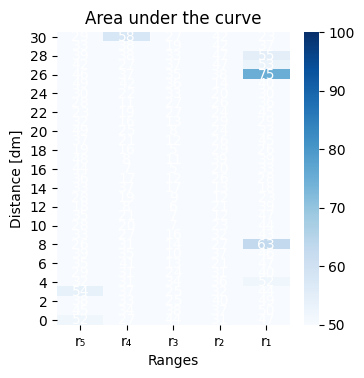
\includegraphics[width=6cm,height=6cm]{4_plots/plots_17/AUC_17.png}
\caption{The left graph shows the validation versus the training loss while the right graph shows the summary of the Area Under the Receiver Operating Characteristic curve for all ranges from $\{r_{1}, ... ,r_{n}\}$ as well for all intermediary positions (distances).}
\label{auc_17}
\end{figure}



\newpage
\subsubsection{Model 19\label{model_19} }
\begin{multicols}{2}\textbf{Data acquisition}
\begin{itemize}
\setlength\itemsep{0.1em}
\item recorded bagfiles: 20
\item recorded images: 1200
\item angle avoidance: 45
\item timeout limit: 20
\item recording distance: 3.0
\item safe passage diameter: 2
\end{itemize}
\textbf{Feature Extraction}
\begin{itemize}
\setlength\itemsep{0.1em}
\item Dataset name: dataset\_19.h5
\item  laser range: 233:437
\item  laser sections: 5
\item  laser count: 666
\item  selection range: 2
\item  target count: 31
\item  laser threshold: 1.0
\end{itemize}
\columnbreak\textbf{Training Model}
\begin{itemize}
\setlength\itemsep{0.1em}
\item  Model name: model\_19.h5
\item  No. of epochs: 15
\item  Steps: 1000
\item  Batch Size: 64
\item  Learning Rate: 0.0002
\item  Ratio val vs training: 0.85
\end{itemize}
\textbf{Testing Model}
\begin{itemize}
\setlength\itemsep{0.1em}
\item Rounds: 100
\newline
\newline
\newline
\newline
\newline
\newline
\newline
\newline
\end{itemize}
\end{multicols}\begin{figure}[H]%[htbp]
\centering
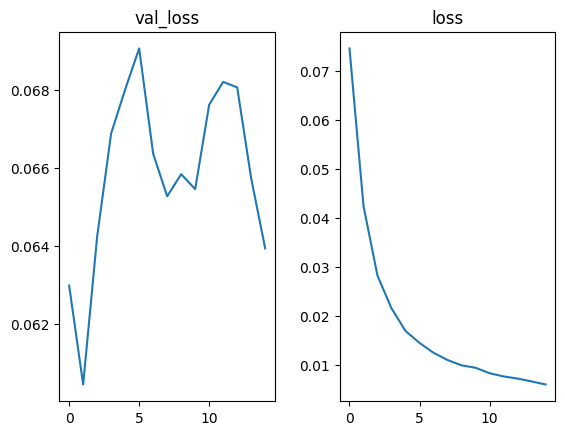
\includegraphics[width=8cm,height=6cm]{3_models/models_19/graph_19.png}
\hspace{0.2 cm}
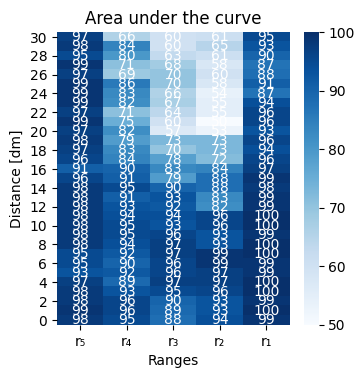
\includegraphics[width=6cm,height=6cm]{4_plots/plots_19/AUC_19.png}
\caption{The left graph shows the validation versus the training loss while the right graph shows the summary of the Area Under the Receiver Operating Characteristic curve for all ranges from $\{r_{1}, ... ,r_{n}\}$ as well for all intermediary positions (distances).}
\label{auc_19}
\end{figure}



\newpage
\subsubsection{Model 20\label{model_20} }
\begin{multicols}{2}\textbf{Data acquisition}
\begin{itemize}
\setlength\itemsep{0.1em}
\item recorded bagfiles: 40
\item recorded images: 2400
\item angle avoidance: 45
\item timeout limit: 20
\item recording distance: 3.0
\item safe passage diameter: 2
\end{itemize}
\textbf{Feature Extraction}
\begin{itemize}
\setlength\itemsep{0.1em}
\item Dataset name: dataset\_20.h5
\item  laser range: 233:437
\item  laser sections: 5
\item  laser count: 666
\item  selection range: 2
\item  target count: 31
\item  laser threshold: 1.0
\end{itemize}
\columnbreak\textbf{Training Model}
\begin{itemize}
\setlength\itemsep{0.1em}
\item  Model name: model\_20.h5
\item  No. of epochs: 15
\item  Steps: 1000
\item  Batch Size: 64
\item  Learning Rate: 0.0002
\item  Ratio val vs training: 0.85
\end{itemize}
\textbf{Testing Model}
\begin{itemize}
\setlength\itemsep{0.1em}
\item Rounds: 100
\newline
\newline
\newline
\newline
\newline
\newline
\newline
\newline
\end{itemize}
\end{multicols}\begin{figure}[H]%[htbp]
\centering
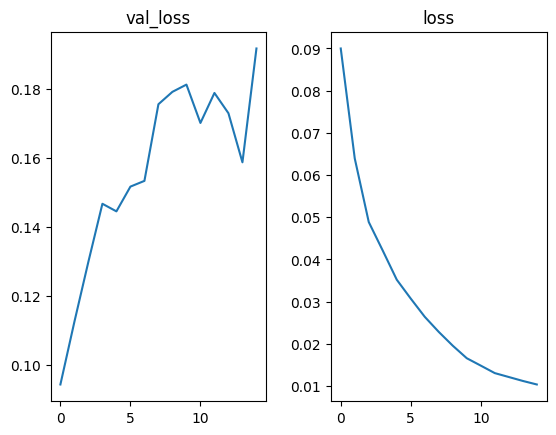
\includegraphics[width=8cm,height=6cm]{3_models/models_20/graph_20.png}
\hspace{0.2 cm}
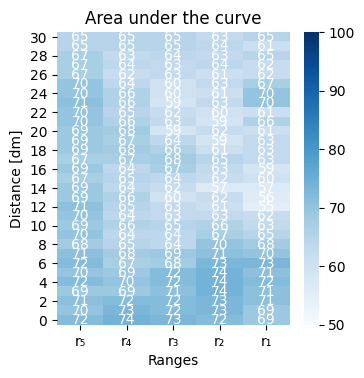
\includegraphics[width=6cm,height=6cm]{4_plots/plots_20/AUC_20.png}
\caption{The left graph shows the validation versus the training loss while the right graph shows the summary of the Area Under the Receiver Operating Characteristic curve for all ranges from $\{r_{1}, ... ,r_{n}\}$ as well for all intermediary positions (distances).}
\label{auc_20}
\end{figure}


\newpage
\subsubsection{Model 25\label{model_25} }
\begin{multicols}{2}\textbf{Data acquisition}
\begin{itemize}
\setlength\itemsep{0.1em}
\item recorded bagfiles: 80
\item recorded images: 4800
\item angle avoidance: 89
\item timeout limit: 20
\item recording distance: 3.0
\item safe passage diameter: 2
\end{itemize}
\textbf{Feature Extraction}
\begin{itemize}
\setlength\itemsep{0.1em}
\item Dataset name: dataset\_25.h5
\item  laser range: 233:437
\item  laser sections: 5
\item  laser count: 666
\item  selection range: 2
\item  target count: 31
\item  laser threshold: 1.35
\end{itemize}
\columnbreak\textbf{Training Model}
\begin{itemize}
\setlength\itemsep{0.1em}
\item  Model name: model\_25.h5
\item  No. of epochs: 15
\item  Steps: 1000
\item  Batch Size: 64
\item  Learning Rate: 0.0002
\item  Ratio val vs training: 0.85
\end{itemize}
\textbf{Testing Model}
\begin{itemize}
\setlength\itemsep{0.1em}
\item Rounds: 100
\newline
\newline
\newline
\newline
\newline
\newline
\newline
\newline
\end{itemize}
\end{multicols}\begin{figure}[H]%[htbp]
\centering
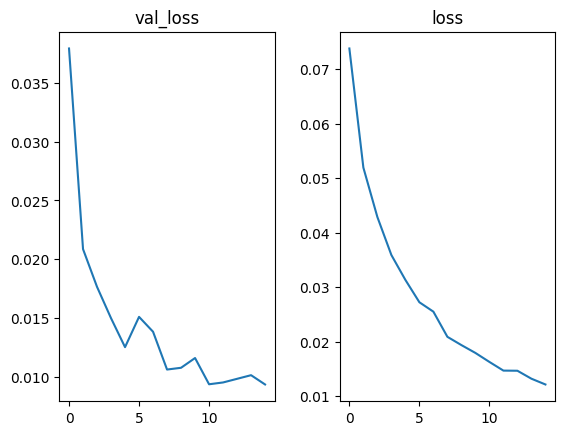
\includegraphics[width=8cm,height=6cm]{3_models/models_25/graph_25.png}
\hspace{0.2 cm}
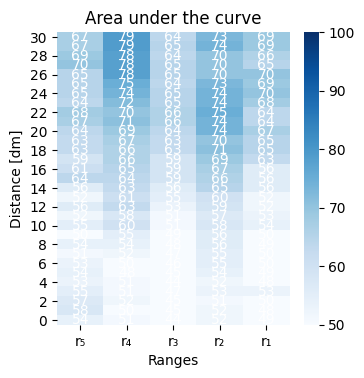
\includegraphics[width=6cm,height=6cm]{4_plots/plots_25/AUC_25.png}
\caption{The left graph shows the validation versus the training loss while the right graph shows the summary of the Area Under the Receiver Operating Characteristic curve for all ranges from $\{r_{1}, ... ,r_{n}\}$ as well for all intermediary positions (distances).}
\label{auc_25}
\end{figure}
\newpage


\newpage
\subsubsection{Model 26\label{model_26} }
\begin{multicols}{2}\textbf{Data acquisition}
\begin{itemize}
\setlength\itemsep{0.1em}
\item recorded bagfiles: 160
\item recorded images: 9600
\item angle avoidance: random int
\item timeout limit: 20
\item recording distance: 3.0
\item safe passage diameter: 2
\end{itemize}
\textbf{Feature Extraction}
\begin{itemize}
\setlength\itemsep{0.1em}
\item Dataset name: dataset\_26.h5
\item  laser range: 233:437
\item  laser sections: 5
\item  laser count: 666
\item  selection range: 2
\item  target count: 31
\item  laser threshold: 1.35
\end{itemize}
\columnbreak\textbf{Training Model}
\begin{itemize}
\setlength\itemsep{0.1em}
\item  Model name: model\_26.h5
\item  No. of epochs: 15
\item  Steps: 1000
\item  Batch Size: 64
\item  Learning Rate: 0.0002
\item  Ratio val vs training: 0.85
\end{itemize}
\textbf{Testing Model}
\begin{itemize}
\setlength\itemsep{0.1em}
\item Rounds: 100
\newline
\newline
\newline
\newline
\newline
\newline
\newline
\newline
\end{itemize}
\end{multicols}\begin{figure}[H]%[htbp]
\centering
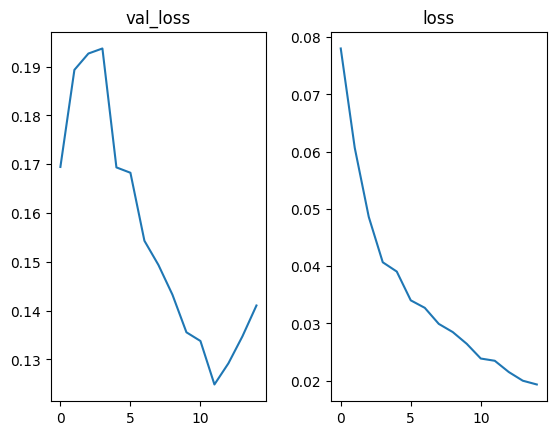
\includegraphics[width=8cm,height=6cm]{3_models/models_26/graph_26.png}
\hspace{0.2 cm}
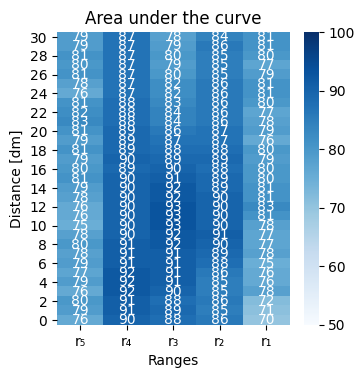
\includegraphics[width=6cm,height=6cm]{4_plots/plots_26/AUC_26.png}
\caption{The left graph shows the validation versus the training loss while the right graph shows the summary of the Area Under the Receiver Operating Characteristic curve for all ranges from $\{r_{1}, ... ,r_{n}\}$ as well for all intermediary positions (distances).}
\label{auc_26}
\end{figure}


\newpage
\subsubsection{Model 27\label{model_27} }
\begin{multicols}{2}\textbf{Data acquisition}
\begin{itemize}
\setlength\itemsep{0.1em}
\item recorded bagfiles: 160
\item recorded images: 9600
\item angle avoidance: random int
\item timeout limit: 20
\item recording distance: 3.0
\item safe passage diameter: 2
\end{itemize}
\textbf{Feature Extraction}
\begin{itemize}
\setlength\itemsep{0.1em}
\item Dataset name: dataset\_26.h5
\item  laser range: 233:437
\item  laser sections: 5
\item  laser count: 666
\item  selection range: 2
\item  target count: 31
\item  laser threshold: 1.35
\end{itemize}
\columnbreak\textbf{Training Model}
\begin{itemize}
\setlength\itemsep{0.1em}
\item  Model name: model\_27.h5
\item  No. of epochs: 15
\item  Steps: 1000
\item  Batch Size: 64
\item  Learning Rate: 0.002
\item  Ratio val vs training: 0.85
\end{itemize}
\textbf{Testing Model}
\begin{itemize}
\setlength\itemsep{0.1em}
\item Rounds: 100
\newline
\newline
\newline
\newline
\newline
\newline
\newline
\newline
\end{itemize}
\end{multicols}\begin{figure}[H]%[htbp]
\centering
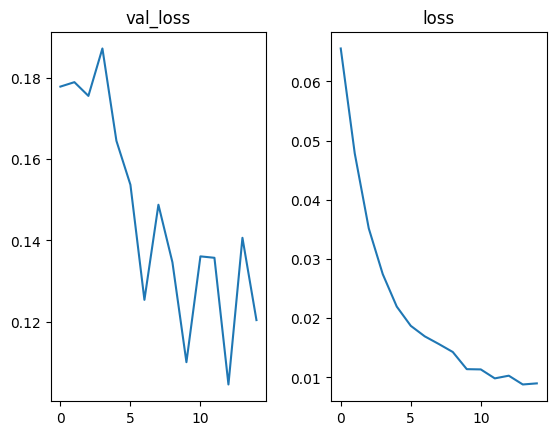
\includegraphics[width=8cm,height=6cm]{3_models/models_27/graph_27.png}
\hspace{0.2 cm}
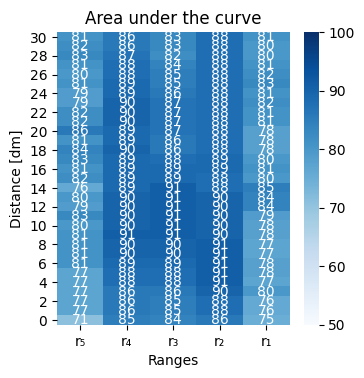
\includegraphics[width=6cm,height=6cm]{4_plots/plots_27/AUC_27.png}
\caption{The left graph shows the validation versus the training loss while the right graph shows the summary of the Area Under the Receiver Operating Characteristic curve for all ranges from $\{r_{1}, ... ,r_{n}\}$ as well for all intermediary positions (distances).}
\label{auc_27}
\end{figure}


\newpage
\subsubsection{Model 28\label{model_28} }
\begin{multicols}{2}\textbf{Data acquisition}
\begin{itemize}
\setlength\itemsep{0.1em}
\item recorded bagfiles: 160
\item recorded images: 9600
\item angle avoidance: random int
\item timeout limit: 20
\item recording distance: 3.0
\item safe passage diameter: 2
\end{itemize}
\textbf{Feature Extraction}
\begin{itemize}
\setlength\itemsep{0.1em}
\item Dataset name: dataset\_26.h5
\item  laser range: 233:437
\item  laser sections: 5
\item  laser count: 666
\item  selection range: 2
\item  target count: 31
\item  laser threshold: 1.35
\end{itemize}
\columnbreak\textbf{Training Model}
\begin{itemize}
\setlength\itemsep{0.1em}
\item  Model name: model\_28.h5
\item  No. of epochs: 15
\item  Steps: 1000
\item  Batch Size: 64
\item  Learning Rate: 0.0004
\item  Ratio val vs training: 0.85
\end{itemize}
\textbf{Testing Model}
\begin{itemize}
\setlength\itemsep{0.1em}
\item Rounds: 100
\newline
\newline
\newline
\newline
\newline
\newline
\newline
\newline
\end{itemize}
\end{multicols}\begin{figure}[H]%[htbp]
\centering
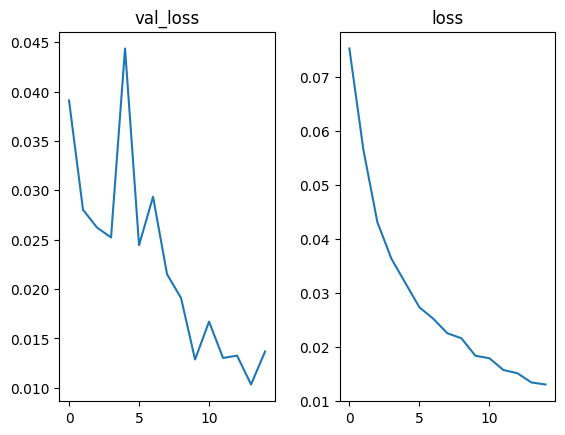
\includegraphics[width=8cm,height=6cm]{3_models/models_28/graph_28.png}
\hspace{0.2 cm}
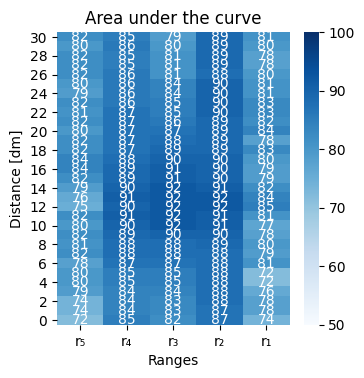
\includegraphics[width=6cm,height=6cm]{4_plots/plots_28/AUC_28.png}
\caption{The left graph shows the validation versus the training loss while the right graph shows the summary of the Area Under the Receiver Operating Characteristic curve for all ranges from $\{r_{1}, ... ,r_{n}\}$ as well for all intermediary positions (distances).}
\label{auc_28}
\end{figure}



\subsubsection{Summary\label{summary_batch_3} }
Table \ref{tab:summary_table_3} displays the summary of this batch. The tests are defined in Section 4.4.3 in the main paper. The table contains following information:
\begin{itemize}
\item  \textbf{Laser ranges: }Lowest to highest AUC result defined for each range
\item  \textbf{Unknown obstacles: }Performance result on unknown obstacles as two elements. The first element defines whether the model is able to properly recognize distances, while the second value, represents if ranges are predicted accurately.
\item  \textbf{Correct Distances: }Performance result for distances containing three elements. Each element represents a range of 1 meter starting with the first element from 0m to 1m with all subsequent elements alike.
\item  \textbf{Empty instances: }Result whether empty instance are recognized or not
\item  \textbf{Correct range: }Performance result for correct ranges to be recognized
\item  \textbf{Images recorded: }Amount of images recorded
\end{itemize}



\begin{table}[H]
\resizebox{\columnwidth}{!}{%
\begin{tabular}{|c|c|c|c|c|c|c|c|c|c|c|c|}
\hline
\rowcolor[HTML]{020B36} 
{\color[HTML]{FFFFFF} \textbf{\begin{tabular}[c]{@{}c@{}}Model\\ name\end{tabular}}} & {\color[HTML]{FFFFFF} \textbf{$r_{5}$}} & {\color[HTML]{FFFFFF} \textbf{$r_{4}$}} & {\color[HTML]{FFFFFF} \textbf{$r_{3}$}} & {\color[HTML]{FFFFFF} \textbf{$r_{2}$}} & {\color[HTML]{FFFFFF} \textbf{$r_{1}$}} & {\color[HTML]{FFFFFF} \textbf{\begin{tabular}[c]{@{}c@{}}Learning\\ rate\end{tabular}}} & {\color[HTML]{FFFFFF} \textbf{\begin{tabular}[c]{@{}c@{}}Unknown\\ obstacles\end{tabular}}} & {\color[HTML]{FFFFFF} \textbf{\begin{tabular}[c]{@{}c@{}}Correct\\ distances\end{tabular}}} & {\color[HTML]{FFFFFF} \textbf{\begin{tabular}[c]{@{}c@{}}Empty\\ instances\end{tabular}}} & {\color[HTML]{FFFFFF} \textbf{\begin{tabular}[c]{@{}c@{}}Correct\\ range\end{tabular}}} & {\color[HTML]{FFFFFF} \textbf{\begin{tabular}[c]{@{}c@{}}Images\\ recorded\end{tabular}}} \\ \hline
\rowcolor[HTML]{FFFFFF} 
$M_{17}$                                                                             & 50 - 54                                 & 50 - 58                                 & 50 - 50                                 & 50 - 50                                 & 50 - 75                                 & .0002                                                                                   & {[}0,0{]}                                                                                   & {[}0,0,.2{]}                                                                                & no                                                                                        & {[}0,0,0,0,0{]}                                                                         & 600                                                                                       \\ \hline
\rowcolor[HTML]{FFFFFF} 
$M_{19}$                                                                             & 93 - 99                                 & 66  - 96                                & 57 - 95                                 & 50 - 99                                 & 87 100                                  & .0002                                                                                   & {[}0,0{]}                                                                                   & {[}0,0,0{]}                                                                                 & no                                                                                        & {[}.2,.2,.2,.2,.2{]}                                                                    & 1200                                                                                      \\ \hline
\rowcolor[HTML]{FFFFFF} 
$M_{20}$                                                                             & 65 - 71                                 & 64 - 74                                 & 60 - 73                                 & 59 - 74                                 & 61 - 73                                 & .0002                                                                                   & {[}0,0{]}                                                                                   & {[}0,0,0{]}                                                                                 & yes                                                                                       & {[}.2,.2,.2,.2,.2{]}                                                                    & 2400                                                                                      \\ \hline
\rowcolor[HTML]{FFFFFF} 
$M_{25}$                                                                             & 50 - 70                                 & 50 - 79                                 & 50 - 65                                 & 52 - 74                                 & 50 70                                   & .0002                                                                                   & {[}0,1{]}                                                                                   & {[}0,0.4,0.8{]}                                                                             & yes                                                                                       & {[}.5,.5,.5,.5,.5{]}                                                                    & 4800                                                                                      \\ \hline
\rowcolor[HTML]{FFFFFF} 
$M_{26}$                                                                             & 76 - 83                                 & 87 - 90                                 & 78 - 91                                 & 84 90                                   & 70 - 83                                 & .0002                                                                                   & {[}0,0{]}                                                                                   & {[}0,.6,.9{]}                                                                               & yes                                                                                       & {[}.8,.9,.9,.9,.6{]}                                                                    & 9600                                                                                      \\ \hline
\rowcolor[HTML]{FFFFFF} 
$M_{27}$                                                                             & 71 - 86                                 & 86 - 91                                 & 82 - 91                                 & 86 - 91                                 & 78 - 85                                 & .002                                                                                    & {[}0,3{]}                                                                                   & {[}0,.5,.9{]}                                                                               & yes                                                                                       & {[}.6,.8,.8,.8,.5{]}                                                                    & 9600                                                                                      \\ \hline
\rowcolor[HTML]{FFFFFF} 
$M_{28}$                                                                             & 72 - 84                                 & 85 - 91                                 & 79 - 91                                 & 87 - 92                                 & 72 - 83                                 & .0004                                                                                   & {[}0,3{]}                                                                                   & {[}0,.4,.9{]}                                                                               & yes                                                                                       & {[}.6,.7,.7,.7,.5{]}                                                                    & 9600                                                                                      \\ \hline
\end{tabular}
}
\caption{Summary table}
\label{tab:summary_table_3}
\end{table}


\newpage

\subsection{Batch 4 \label{batch_4} }
These are the test results for the fourth training batch, which consists of 5 different models with the number of images increased from 1540 to 12320. \figref{env4} displays the environment used for this batch.

\begin{figure}[H]%[htbp]
\centering
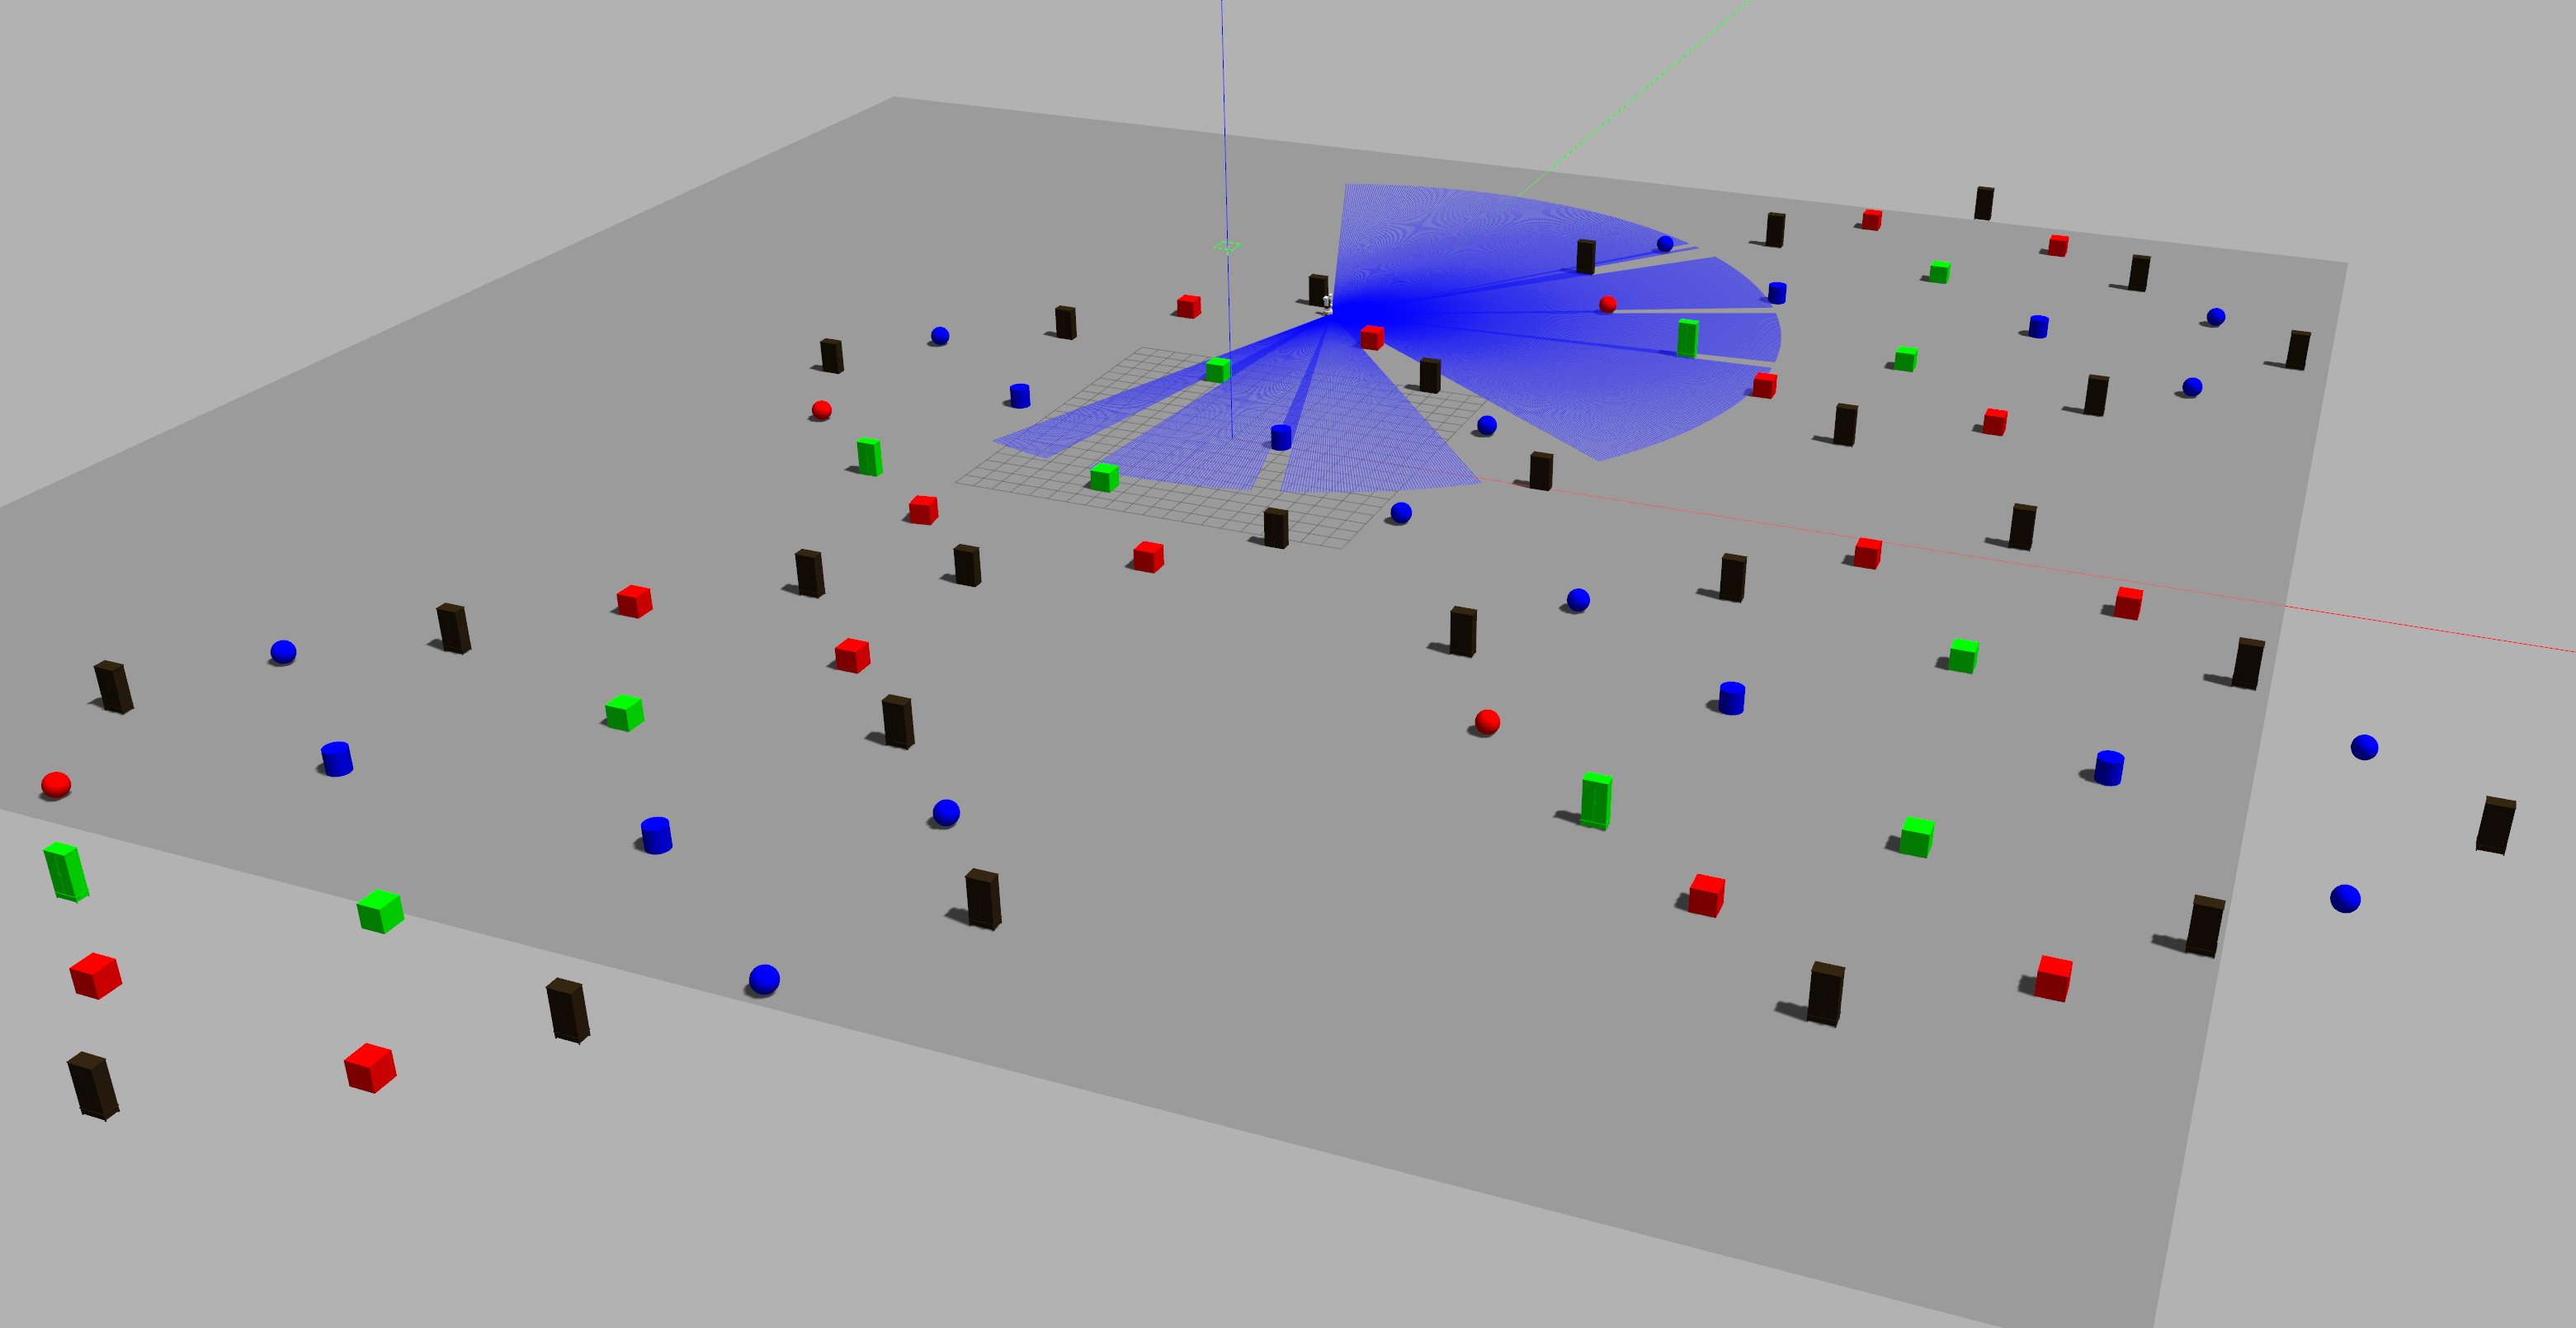
\includegraphics[width=1\textwidth]{Bilder/env5.png} 
\caption[]{Environment used for Batch 4.}
\label{env5}
\end{figure}

The following subsections, will list the parameters and graphs used for each model created by the pipeline. The manual test results, as defined in Section 4.4.3 in the main paper, are summarized in \secref{summary_batch_3}.


\newpage
\subsubsection{Model 29\label{model_29} }
\begin{multicols}{2}\textbf{Data acquisition}
\begin{itemize}
\setlength\itemsep{0.1em}
\item recorded bagfiles: 10
\item recorded images: 1540
\item angle avoidance: random int
\item timeout limit: 20
\item recording distance: 8.0
\item safe passage diameter: 2
\end{itemize}
\textbf{Feature Extraction}
\begin{itemize}
\setlength\itemsep{0.1em}
\item Dataset name: dataset\_29.h5
\item  laser range: 233:437
\item  laser sections: 5
\item  laser count: 666
\item  selection range: 1
\item  target count: 81
\item  laser threshold: 1.8
\end{itemize}
\columnbreak\textbf{Training Model}
\begin{itemize}
\setlength\itemsep{0.1em}
\item  Model name: model\_29.h5
\item  No. of epochs: 15
\item  Steps: 1000
\item  Batch Size: 64
\item  Learning Rate: 0.0004
\item  Ratio val vs training: 0.85
\end{itemize}
\textbf{Testing Model}
\begin{itemize}
\setlength\itemsep{0.1em}
\item Rounds: 100
\newline
\newline
\newline
\newline
\newline
\newline
\newline
\newline
\end{itemize}
\end{multicols}\begin{figure}[H]%[htbp]
\centering
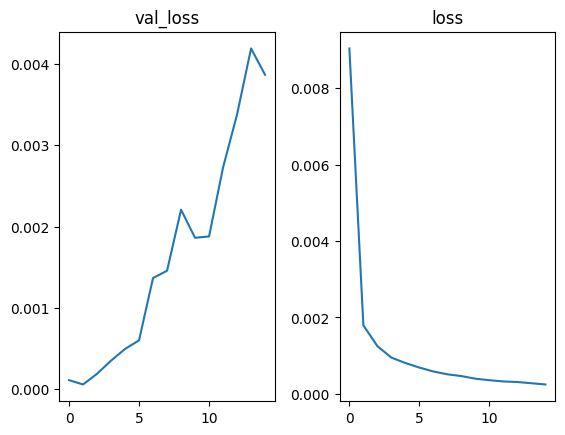
\includegraphics[width=8cm,height=6cm]{3_models/models_29/graph_29.png}
\hspace{0.2 cm}
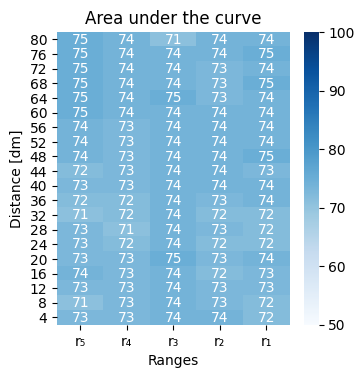
\includegraphics[width=6cm,height=6cm]{4_plots/plots_29/AUC_29.png}
\caption{The left graph shows the validation versus the training loss while the right graph shows the summary of the Area Under the Receiver Operating Characteristic curve for all ranges from $\{r_{1}, ... ,r_{n}\}$ as well for all intermediary positions (distances).}
\label{auc_29}
\end{figure}



\newpage
\subsubsection{Model 30\label{model_30} }
\begin{multicols}{2}\textbf{Data acquisition}
\begin{itemize}
\setlength\itemsep{0.1em}
\item recorded bagfiles: 20
\item recorded images: 3120
\item angle avoidance: random int
\item timeout limit: 20
\item recording distance: 8.0
\item safe passage diameter: 2
\end{itemize}
\textbf{Feature Extraction}
\begin{itemize}
\setlength\itemsep{0.1em}
\item Dataset name: dataset\_30.h5
\item  laser range: 233:437
\item  laser sections: 5
\item  laser count: 666
\item  selection range: 1
\item  target count: 81
\item  laser threshold: 1.8
\end{itemize}
\columnbreak\textbf{Training Model}
\begin{itemize}
\setlength\itemsep{0.1em}
\item  Model name: model\_30.h5
\item  No. of epochs: 15
\item  Steps: 1000
\item  Batch Size: 64
\item  Learning Rate: 0.0004
\item  Ratio val vs training: 0.85
\end{itemize}
\textbf{Testing Model}
\begin{itemize}
\setlength\itemsep{0.1em}
\item Rounds: 100
\newline
\newline
\newline
\newline
\newline
\newline
\newline
\newline
\end{itemize}
\end{multicols}\begin{figure}[H]%[htbp]
\centering
\includegraphics[width=8cm,height=6cm]{3_models/models_30/graph_30.png}
\hspace{0.2 cm}
\includegraphics[width=6cm,height=6cm]{4_plots/plots_30/AUC_30.png}
\caption{The left graph shows the validation versus the training loss while the right graph shows the summary of the Area Under the Receiver Operating Characteristic curve for all ranges from $\{r_{1}, ... ,r_{n}\}$ as well for all intermediary positions (distances).}
\label{auc_30}
\end{figure}


\newpage
\subsubsection{Model 31\label{model_31} }
\begin{multicols}{2}\textbf{Data acquisition}
\begin{itemize}
\setlength\itemsep{0.1em}
\item recorded bagfiles: 40
\item recorded images: 6160
\item angle avoidance: random int
\item timeout limit: 20
\item recording distance: 8.0
\item safe passage diameter: 2
\end{itemize}
\textbf{Feature Extraction}
\begin{itemize}
\setlength\itemsep{0.1em}
\item Dataset name: dataset\_31.h5
\item  laser range: 233:437
\item  laser sections: 5
\item  laser count: 666
\item  selection range: 1
\item  target count: 81
\item  laser threshold: 1.8
\end{itemize}
\columnbreak\textbf{Training Model}
\begin{itemize}
\setlength\itemsep{0.1em}
\item  Model name: model\_31.h5
\item  No. of epochs: 15
\item  Steps: 1000
\item  Batch Size: 64
\item  Learning Rate: 0.0004
\item  Ratio val vs training: 0.85
\end{itemize}
\textbf{Testing Model}
\begin{itemize}
\setlength\itemsep{0.1em}
\item Rounds: 100
\newline
\newline
\newline
\newline
\newline
\newline
\newline
\newline
\end{itemize}
\end{multicols}\begin{figure}[H]%[htbp]
\centering
\includegraphics[width=8cm,height=6cm]{3_models/models_31/graph_31.png}
\hspace{0.2 cm}
\includegraphics[width=6cm,height=6cm]{4_plots/plots_31/AUC_31.png}
\caption{The left graph shows the validation versus the training loss while the right graph shows the summary of the Area Under the Receiver Operating Characteristic curve for all ranges from $\{r_{1}, ... ,r_{n}\}$ as well for all intermediary positions (distances).}
\label{auc_31}
\end{figure}



\newpage
\subsubsection{Model 39\label{model_39} }
\begin{multicols}{2}\textbf{Data acquisition}
\begin{itemize}
\setlength\itemsep{0.1em}
\item recorded bagfiles: 80
\item recorded images: 12320
\item angle avoidance: random int
\item timeout limit: 20
\item recording distance: 8.0
\item safe passage diameter: 2
\end{itemize}
\textbf{Feature Extraction}
\begin{itemize}
\setlength\itemsep{0.1em}
\item Dataset name: dataset\_39.h5
\item  laser range: 233:437
\item  laser sections: 5
\item  laser count: 666
\item  selection range: 1
\item  target count: 81
\item  laser threshold: 1.8
\end{itemize}
\columnbreak\textbf{Training Model}
\begin{itemize}
\setlength\itemsep{0.1em}
\item  Model name: model\_39.h5
\item  No. of epochs: 15
\item  Steps: 1000
\item  Batch Size: 64
\item  Learning Rate: 0.0004
\item  Ratio val vs training: 0.85
\end{itemize}
\textbf{Testing Model}
\begin{itemize}
\setlength\itemsep{0.1em}
\item Rounds: 100
\newline
\newline
\newline
\newline
\newline
\newline
\newline
\newline
\end{itemize}
\end{multicols}\begin{figure}[H]%[htbp]
\centering
\includegraphics[width=8cm,height=6cm]{3_models/models_39/graph_39.png}
\hspace{0.2 cm}
\includegraphics[width=6cm,height=6cm]{4_plots/plots_39/AUC_39.png}
\caption{The left graph shows the validation versus the training loss while the right graph shows the summary of the Area Under the Receiver Operating Characteristic curve for all ranges from $\{r_{1}, ... ,r_{n}\}$ as well for all intermediary positions (distances).}
\label{auc_39}
\end{figure}


\newpage


\subsubsection{Summary\label{summary_batch_4} }
Table \ref{tab:summary_table_4} displays the summary of this batch. The tests are defined in Section 4.4.3 in the main paper. The table contains following information:
\begin{itemize}
\item  \textbf{Laser ranges: }Lowest to highest AUC result defined for each range
\item  \textbf{Unknown obstacles: }Performance result on unknown obstacles as two elements. The first element defines whether the model is able to properly recognize distances, while the second value, represents if ranges are predicted accurately.
\item  \textbf{Correct Distances: }Performance result for distances containing three elements. Each element represents a range of 1 meter starting with the first element from 0m to 1m with all subsequent elements alike.
\item  \textbf{Empty instances: }Result whether empty instance are recognized or not
\item  \textbf{Correct range: }Performance result for correct ranges to be recognized
\item  \textbf{Images recorded: }Amount of images recorded
\end{itemize}

\begin{table}[H]
\resizebox{\columnwidth}{!}{%
\begin{tabular}{|c|c|c|c|c|c|c|c|c|c|c|c|}
\hline
\rowcolor[HTML]{020B36} 
{\color[HTML]{FFFFFF} \textbf{\begin{tabular}[c]{@{}c@{}}Model\\ name\end{tabular}}} & {\color[HTML]{FFFFFF} \textbf{$r_{5}$}} & {\color[HTML]{FFFFFF} \textbf{$r_{4}$}} & {\color[HTML]{FFFFFF} \textbf{$r_{3}$}} & {\color[HTML]{FFFFFF} \textbf{$r_{2}$}} & {\color[HTML]{FFFFFF} \textbf{$r_{1}$}} & {\color[HTML]{FFFFFF} \textbf{\begin{tabular}[c]{@{}c@{}}Learning\\ rate\end{tabular}}} & {\color[HTML]{FFFFFF} \textbf{\begin{tabular}[c]{@{}c@{}}Unknown\\ obstacles\end{tabular}}} & {\color[HTML]{FFFFFF} \textbf{\begin{tabular}[c]{@{}c@{}}Correct\\ distances\end{tabular}}} & {\color[HTML]{FFFFFF} \textbf{\begin{tabular}[c]{@{}c@{}}Empty\\ instances\end{tabular}}} & {\color[HTML]{FFFFFF} \textbf{\begin{tabular}[c]{@{}c@{}}Correct\\ range\end{tabular}}} & {\color[HTML]{FFFFFF} \textbf{\begin{tabular}[c]{@{}c@{}}Images\\ recorded\end{tabular}}} \\ \hline
\rowcolor[HTML]{FFFFFF} 
$M_{29}$                                                                             & 71 - 75                                 & 71 - 74                                 & 71 - 75                                 & 72 - 74                                 & 72 - 75                                 & .0004                                                                                   & {[}.2,.3{]}                                                                                 & {[}0,.3,.1{]}                                                                               & yes                                                                                       & {[}.1,.1,.1,.1,.1{]}                                                                    & 1540                                                                                      \\ \hline
\rowcolor[HTML]{FFFFFF} 
$M_{30}$                                                                             & 70 - 83                                 & 81 - 83                                 & 81 - 83                                 & 81 - 83                                 & 79 - 83                                 & .0004                                                                                   & {[}.4,.5{]}                                                                                 & {[}0,.6,.4{]}                                                                               & yes                                                                                       & {[}.4,.5,.8,.5,.4{]}                                                                    & 3120                                                                                      \\ \hline
\rowcolor[HTML]{FFFFFF} 
$M_{31}$                                                                             & 83 - 90                                 & 94 - 99                                 & 60 - 73                                 & 59 - 74                                 & 61 - 73                                 & .0004                                                                                   & {[}.2,.8{]}                                                                                 & {[}0,.5,.4{]}                                                                               & yes                                                                                       & {[}.2,.5,.8,.5,.2{]}                                                                    & 6160                                                                                      \\ \hline
\rowcolor[HTML]{FFFFFF} 
$M_{39}$                                                                             & 50 - 50                                 & 50 - 50                                 & 50 - 50                                 & 50 - 50                                 & 50 - 50                                 & .0004                                                                                   & {[}.0,.0{]}                                                                                 & {[}0,.0,.0{]}                                                                               & no                                                                                        & {[}.0,.0,.0,.0,.0{]}                                                                    & 12320                                                                                     \\ \hline
\end{tabular}
}
\caption{Summary table}
\label{tab:summary_table_4}
\end{table}

\newpage

\subsection{Batch 5 \label{batch_5} }
These are the test results for the fourth training batch, which consists of 5 different models with the number of images increased from 730 to 12410. \figref{env4} displays the environment used for this batch.

\begin{figure}[H]%[htbp]
\centering
\includegraphics[width=1\textwidth]{Bilder/env5.png} 
\caption[]{Environment used for Batch 4.}
\label{env5}
\end{figure}

The following subsections, will list the parameters and graphs used for each model created by the pipeline. The manual test results, as defined in Section 4.4.3 in the main paper, are summarized in \secref{summary_batch_4}.

\newpage
\subsubsection{Model 41\label{model_41} }
\begin{multicols}{2}\textbf{Data acquisition}
\begin{itemize}
\setlength\itemsep{0.1em}
\item recorded bagfiles: 10
\item recorded images: 730
\item angle avoidance: random int
\item timeout limit: 20
\item recording distance: 4.0
\item safe passage diameter: 2
\end{itemize}
\textbf{Feature Extraction}
\begin{itemize}
\setlength\itemsep{0.1em}
\item Dataset name: dataset\_41.h5
\item  laser range: 233:437
\item  laser sections: 5
\item  laser count: 666
\item  selection range: 1
\item  target count: 41
\item  laser threshold: 1.4
\end{itemize}
\columnbreak\textbf{Training Model}
\begin{itemize}
\setlength\itemsep{0.1em}
\item  Model name: model\_41.h5
\item  No. of epochs: 15
\item  Steps: 1000
\item  Batch Size: 64
\item  Learning Rate: 0.0004
\item  Ratio val vs training: 0.85
\end{itemize}
\textbf{Testing Model}
\begin{itemize}
\setlength\itemsep{0.1em}
\item Rounds: 100
\newline
\newline
\newline
\newline
\newline
\newline
\newline
\newline
\end{itemize}
\end{multicols}\begin{figure}[H]%[htbp]
\centering
\includegraphics[width=8cm,height=6cm]{3_models/models_41/graph_41.png}
\hspace{0.2 cm}
\includegraphics[width=6cm,height=6cm]{4_plots/plots_41/AUC_41.png}
\caption{The left graph shows the validation versus the training loss while the right graph shows the summary of the Area Under the Receiver Operating Characteristic curve for all ranges from $\{r_{1}, ... ,r_{n}\}$ as well for all intermediary positions (distances).}
\label{auc_41}
\end{figure}


\newpage
\subsubsection{Model 42\label{model_42} }
\begin{multicols}{2}\textbf{Data acquisition}
\begin{itemize}
\setlength\itemsep{0.1em}
\item recorded bagfiles: 20
\item recorded images: 1460
\item angle avoidance: random int
\item timeout limit: 20
\item recording distance: 4.0
\item safe passage diameter: 2
\end{itemize}
\textbf{Feature Extraction}
\begin{itemize}
\setlength\itemsep{0.1em}
\item Dataset name: dataset\_42.h5
\item  laser range: 233:437
\item  laser sections: 5
\item  laser count: 666
\item  selection range: 1
\item  target count: 41
\item  laser threshold: 1.4
\end{itemize}
\columnbreak\textbf{Training Model}
\begin{itemize}
\setlength\itemsep{0.1em}
\item  Model name: model\_42.h5
\item  No. of epochs: 15
\item  Steps: 1000
\item  Batch Size: 64
\item  Learning Rate: 0.0004
\item  Ratio val vs training: 0.85
\end{itemize}
\textbf{Testing Model}
\begin{itemize}
\setlength\itemsep{0.1em}
\item Rounds: 100
\newline
\newline
\newline
\newline
\newline
\newline
\newline
\newline
\end{itemize}
\end{multicols}\begin{figure}[H]%[htbp]
\centering
\includegraphics[width=8cm,height=6cm]{3_models/models_42/graph_42.png}
\hspace{0.2 cm}
\includegraphics[width=6cm,height=6cm]{4_plots/plots_42/AUC_42.png}
\caption{The left graph shows the validation versus the training loss while the right graph shows the summary of the Area Under the Receiver Operating Characteristic curve for all ranges from $\{r_{1}, ... ,r_{n}\}$ as well for all intermediary positions (distances).}
\label{auc_42}
\end{figure}


\newpage
\subsubsection{Model 43\label{model_43} }
\begin{multicols}{2}\textbf{Data acquisition}
\begin{itemize}
\setlength\itemsep{0.1em}
\item recorded bagfiles: 40
\item recorded images: 2920
\item angle avoidance: random int
\item timeout limit: 20
\item recording distance: 4.0
\item safe passage diameter: 2
\end{itemize}
\textbf{Feature Extraction}
\begin{itemize}
\setlength\itemsep{0.1em}
\item Dataset name: dataset\_43.h5
\item  laser range: 233:437
\item  laser sections: 5
\item  laser count: 666
\item  selection range: 1
\item  target count: 41
\item  laser threshold: 1.4
\end{itemize}
\columnbreak\textbf{Training Model}
\begin{itemize}
\setlength\itemsep{0.1em}
\item  Model name: model\_43.h5
\item  No. of epochs: 15
\item  Steps: 1000
\item  Batch Size: 64
\item  Learning Rate: 0.0004
\item  Ratio val vs training: 0.85
\end{itemize}
\textbf{Testing Model}
\begin{itemize}
\setlength\itemsep{0.1em}
\item Rounds: 100
\newline
\newline
\newline
\newline
\newline
\newline
\newline
\newline
\end{itemize}
\end{multicols}\begin{figure}[H]%[htbp]
\centering
\includegraphics[width=8cm,height=6cm]{3_models/models_43/graph_43.png}
\hspace{0.2 cm}
\includegraphics[width=6cm,height=6cm]{4_plots/plots_43/AUC_43.png}
\caption{The left graph shows the validation versus the training loss while the right graph shows the summary of the Area Under the Receiver Operating Characteristic curve for all ranges from $\{r_{1}, ... ,r_{n}\}$ as well for all intermediary positions (distances).}
\label{auc_43}
\end{figure}


\newpage
\subsubsection{Model 44\label{model_44} }
\begin{multicols}{2}\textbf{Data acquisition}
\begin{itemize}
\setlength\itemsep{0.1em}
\item recorded bagfiles: 80
\item recorded images: 5840
\item angle avoidance: random int
\item timeout limit: 20
\item recording distance: 4.0
\item safe passage diameter: 2
\end{itemize}
\textbf{Feature Extraction}
\begin{itemize}
\setlength\itemsep{0.1em}
\item Dataset name: dataset\_44.h5
\item  laser range: 233:437
\item  laser sections: 5
\item  laser count: 666
\item  selection range: 1
\item  target count: 41
\item  laser threshold: 1.4
\end{itemize}
\columnbreak\textbf{Training Model}
\begin{itemize}
\setlength\itemsep{0.1em}
\item  Model name: model\_44.h5
\item  No. of epochs: 15
\item  Steps: 1000
\item  Batch Size: 64
\item  Learning Rate: 0.0004
\item  Ratio val vs training: 0.85
\end{itemize}
\textbf{Testing Model}
\begin{itemize}
\setlength\itemsep{0.1em}
\item Rounds: 100
\newline
\newline
\newline
\newline
\newline
\newline
\newline
\newline
\end{itemize}
\end{multicols}\begin{figure}[H]%[htbp]
\centering
\includegraphics[width=8cm,height=6cm]{3_models/models_44/graph_44.png}
\hspace{0.2 cm}
\includegraphics[width=6cm,height=6cm]{4_plots/plots_44/AUC_44.png}
\caption{The left graph shows the validation versus the training loss while the right graph shows the summary of the Area Under the Receiver Operating Characteristic curve for all ranges from $\{r_{1}, ... ,r_{n}\}$ as well for all intermediary positions (distances).}
\label{auc_44}
\end{figure}


\newpage
\subsubsection{Model 45\label{model_45} }
\begin{multicols}{2}\textbf{Data acquisition}
\begin{itemize}
\setlength\itemsep{0.1em}
\item recorded bagfiles: 170
\item recorded images: 12410
\item angle avoidance: random int
\item timeout limit: 20
\item recording distance: 4.0
\item safe passage diameter: 2
\end{itemize}
\textbf{Feature Extraction}
\begin{itemize}
\setlength\itemsep{0.1em}
\item Dataset name: dataset\_45.h5
\item  laser range: 233:437
\item  laser sections: 5
\item  laser count: 666
\item  selection range: 1
\item  target count: 41
\item  laser threshold: 1.4
\end{itemize}
\columnbreak\textbf{Training Model}
\begin{itemize}
\setlength\itemsep{0.1em}
\item  Model name: model\_45.h5
\item  No. of epochs: 15
\item  Steps: 1000
\item  Batch Size: 64
\item  Learning Rate: 0.0004
\item  Ratio val vs training: 0.85
\end{itemize}
\textbf{Testing Model}
\begin{itemize}
\setlength\itemsep{0.1em}
\item Rounds: 100
\newline
\newline
\newline
\newline
\newline
\newline
\newline
\newline
\end{itemize}
\end{multicols}\begin{figure}[H]%[htbp]
\centering
\includegraphics[width=8cm,height=6cm]{3_models/models_45/graph_45.png}
\hspace{0.2 cm}
\includegraphics[width=6cm,height=6cm]{4_plots/plots_45/AUC_45.png}
\caption{The left graph shows the validation versus the training loss while the right graph shows the summary of the Area Under the Receiver Operating Characteristic curve for all ranges from $\{r_{1}, ... ,r_{n}\}$ as well for all intermediary positions (distances).}
\label{auc_45}
\end{figure}



\subsubsection{Summary\label{summary_batch_5} }
Table \ref{tab:summary_table_5} displays the summary of this batch. The tests are defined in Section 4.4.3 in the main paper. The table contains following information:
\begin{itemize}
\item  \textbf{Laser ranges: }Lowest to highest AUC result defined for each range
\item  \textbf{Unknown obstacles: }Performance result on unknown obstacles as two elements. The first element defines whether the model is able to properly recognize distances, while the second value, represents if ranges are predicted accurately.
\item  \textbf{Correct Distances: }Performance result for distances containing three elements. Each element represents a range of 1 meter starting with the first element from 0m to 1m with all subsequent elements alike.
\item  \textbf{Empty instances: }Result whether empty instance are recognized or not
\item  \textbf{Correct range: }Performance result for correct ranges to be recognized
\item  \textbf{Images recorded: }Amount of images recorded
\end{itemize}


\begin{table}[H]
\resizebox{\columnwidth}{!}{%
\begin{tabular}{|c|c|c|c|c|c|c|c|c|c|c|c|}
\hline
\rowcolor[HTML]{020B36} 
{\color[HTML]{FFFFFF} \textbf{\begin{tabular}[c]{@{}c@{}}Model\\ name\end{tabular}}} & {\color[HTML]{FFFFFF} \textbf{$r_{5}$}} & {\color[HTML]{FFFFFF} \textbf{$r_{4}$}} & {\color[HTML]{FFFFFF} \textbf{$r_{3}$}} & {\color[HTML]{FFFFFF} \textbf{$r_{2}$}} & {\color[HTML]{FFFFFF} \textbf{$r_{1}$}} & {\color[HTML]{FFFFFF} \textbf{\begin{tabular}[c]{@{}c@{}}Learning\\ rate\end{tabular}}} & {\color[HTML]{FFFFFF} \textbf{\begin{tabular}[c]{@{}c@{}}Unknown\\ obstacles\end{tabular}}} & {\color[HTML]{FFFFFF} \textbf{\begin{tabular}[c]{@{}c@{}}Correct\\ distances\end{tabular}}} & {\color[HTML]{FFFFFF} \textbf{\begin{tabular}[c]{@{}c@{}}Empty\\ instances\end{tabular}}} & {\color[HTML]{FFFFFF} \textbf{\begin{tabular}[c]{@{}c@{}}Correct\\ range\end{tabular}}} & {\color[HTML]{FFFFFF} \textbf{\begin{tabular}[c]{@{}c@{}}Images\\ recorded\end{tabular}}} \\ \hline
\rowcolor[HTML]{FFFFFF} 
$M_{41}$                                                                             & 50 - 100                                & 50 - 100                                & 50 - 75                                 & 50 - 100                                & 50 - 100                                & .0004                                                                                   & {[}.1,.1{]}                                                                                 & {[}0,.3,.5{]}                                                                               & no                                                                                        & {[}.0,.0,.0,.0,.0{]}                                                                    & 730                                                                                       \\ \hline
\rowcolor[HTML]{FFFFFF} 
$M_{42}$                                                                             & 50 - 66                                 & 50 - 83                                 & 50 - 66                                 & 50 - 82                                 & 50 - 66                                 & .0004                                                                                   & {[}.3,.4{]}                                                                                 & {[}0,.5,.8{]}                                                                               & no                                                                                        & {[}.1,.2,.2,.1,.1{]}                                                                    & 1460                                                                                      \\ \hline
\rowcolor[HTML]{FFFFFF} 
$M_{43}$                                                                             & 50 - 80                                 & 50 - 82                                 & 50 - 83                                 & 50 - 82                                 & 50 - 80                                 & .0004                                                                                   & {[}.4,.6{]}                                                                                 & {[}4,.7,.8{]}                                                                               & partially                                                                                 & {[}.3,.3,.3,.3,.3{]}                                                                    & 2920                                                                                      \\ \hline
\rowcolor[HTML]{FFFFFF} 
$M_{44}$                                                                             & 50 - 83                                 & 50 - 95                                 & 50 - 95                                 & 50 - 95                                 & 50 - 83                                 & .0004                                                                                   & {[}.3,.5{]}                                                                                 & {[}4,.8,.9{]}                                                                               & partially                                                                                 & {[}.4,.5,.5,.4,.4{]}                                                                    & 5840                                                                                      \\ \hline
\rowcolor[HTML]{FFFFFF} 
$M_{45}$                                                                             & 50 - 86                                 & 50 - 95                                 & 50 - 96                                 & 50 - 95                                 & 50 - 87                                 & .0004                                                                                   & {[}.3,.8{]}                                                                                 & {[}4,.8,.9{]}                                                                               & nearly                                                                                    & {[}.3,.6,.8,.6,.3{]}                                                                    & 12410                                                                                     \\ \hline
\end{tabular}
}
\caption{Summary table}
\label{tab:summary_table_5}
\end{table}

\newpage

\subsection{Batch 6 \label{batch_6} }
These are the test results for the sixth and final training batch, which consists of 7 different models with the amount of images increased from 2400 to 13840. \figref{env6} displays the environment used for this batch. While Model 47, 48, 49 and 62 are recorded on a recording distance of 4.0 meters, Model 59,60 and 61 are recorded on a distance of 3.5 meters.

\begin{figure}[H]%[htbp]
\centering
\includegraphics[width=1\textwidth]{Bilder/env6.png} 
\caption[]{Environment used for Batch 6.}
\label{env6}
\end{figure}

The following subsections, will list the parameters and graphs used for each model created by the pipeline. The manual test results, as defined in Section 4.4.3 in the main paper, are summarized in \secref{summary_batch_6}.

\newpage
\subsubsection{Model 47\label{model_47} }
\begin{multicols}{2}\textbf{Data acquisition}
\begin{itemize}
\setlength\itemsep{0.1em}
\item recorded bagfiles: 43
\item recorded images: 3440
\item angle avoidance: random int
\item timeout limit: 20
\item recording distance: 4.0
\item safe passage diameter: 2
\end{itemize}
\textbf{Feature Extraction}
\begin{itemize}
\setlength\itemsep{0.1em}
\item Dataset name: dataset\_47.h5
\item  laser range: 233:437
\item  laser sections: 5
\item  laser count: 666
\item  selection range: 1
\item  target count: 41
\item  laser threshold: 1.4
\end{itemize}
\columnbreak
\textbf{Training Model}
\begin{itemize}
\setlength\itemsep{0.1em}
\item  Model name: model\_62.h5
\item  No. of epochs: 15
\item  Steps: 1000
\item  Batch Size: 64
\item  Learning Rate: 0.0004
\item  Ratio val vs training: 0.85
\end{itemize}
\textbf{Testing Model}
\begin{itemize}
\setlength\itemsep{0.1em}
\item Rounds: 100
\newline
\newline
\newline
\newline
\newline
\newline
\newline
\newline
\end{itemize}
\end{multicols}\begin{figure}[H]%[htbp]
\centering
\includegraphics[width=8cm,height=6cm]{3_models/models_47/graph_47.png}
\hspace{0.2 cm}
\includegraphics[width=6cm,height=6cm]{4_plots/plots_47/AUC_47.png}
\caption{The left graph shows the validation versus the training loss while the right graph shows the summary of the Area Under the Receiver Operating Characteristic curve for all ranges from $\{r_{1}, ... ,r_{n}\}$ as well for all intermediary positions (distances).}
\label{auc_47}
\end{figure}

\newpage
\subsubsection{Model 48\label{model_48} }
\begin{multicols}{2}\textbf{Data acquisition}
\begin{itemize}
\setlength\itemsep{0.1em}
\item recorded bagfiles: 83
\item recorded images: 6640
\item angle avoidance: random int
\item timeout limit: 20
\item recording distance: 4.0
\item safe passage diameter: 2
\end{itemize}
\textbf{Feature Extraction}
\begin{itemize}
\setlength\itemsep{0.1em}
\item Dataset name: dataset\_48.h5
\item  laser range: 233:437
\item  laser sections: 5
\item  laser count: 666
\item  selection range: 1
\item  target count: 41
\item  laser threshold: 1.4
\end{itemize}
\columnbreak
\textbf{Training Model}
\begin{itemize}
\setlength\itemsep{0.1em}
\item  Model name: model\_62.h5
\item  No. of epochs: 15
\item  Steps: 1000
\item  Batch Size: 64
\item  Learning Rate: 0.0004
\item  Ratio val vs training: 0.85
\end{itemize}
\textbf{Testing Model}
\begin{itemize}
\setlength\itemsep{0.1em}
\item Rounds: 100
\newline
\newline
\newline
\newline
\newline
\newline
\newline
\newline
\end{itemize}
\end{multicols}\begin{figure}[H]%[htbp]
\centering
\includegraphics[width=8cm,height=6cm]{3_models/models_48/graph_48.png}
\hspace{0.2 cm}
\includegraphics[width=6cm,height=6cm]{4_plots/plots_48/AUC_48.png}
\caption{The left graph shows the validation versus the training loss while the right graph shows the summary of the Area Under the Receiver Operating Characteristic curve for all ranges from $\{r_{1}, ... ,r_{n}\}$ as well for all intermediary positions (distances).}
\label{auc_48}
\end{figure}

\newpage
\subsubsection{Model 49\label{model_49} }
\begin{multicols}{2}\textbf{Data acquisition}
\begin{itemize}
\setlength\itemsep{0.1em}
\item recorded bagfiles: 173
\item recorded images: 13840
\item angle avoidance: random int
\item timeout limit: 20
\item recording distance: 4.0
\item safe passage diameter: 2
\end{itemize}
\textbf{Feature Extraction}
\begin{itemize}
\setlength\itemsep{0.1em}
\item Dataset name: dataset\_49.h5
\item  laser range: 233:437
\item  laser sections: 5
\item  laser count: 666
\item  selection range: 1
\item  target count: 41
\item  laser threshold: 1.4
\end{itemize}
\columnbreak
\textbf{Training Model}
\begin{itemize}
\setlength\itemsep{0.1em}
\item  Model name: model\_62.h5
\item  No. of epochs: 15
\item  Steps: 1000
\item  Batch Size: 64
\item  Learning Rate: 0.0004
\item  Ratio val vs training: 0.85
\end{itemize}
\textbf{Testing Model}
\begin{itemize}
\setlength\itemsep{0.1em}
\item Rounds: 100
\newline
\newline
\newline
\newline
\newline
\newline
\newline
\newline
\end{itemize}
\end{multicols}\begin{figure}[H]%[htbp]
\centering
\includegraphics[width=8cm,height=6cm]{3_models/models_49/graph_49.png}
\hspace{0.2 cm}
\includegraphics[width=6cm,height=6cm]{4_plots/plots_49/AUC_49.png}
\caption{The left graph shows the validation versus the training loss while the right graph shows the summary of the Area Under the Receiver Operating Characteristic curve for all ranges from $\{r_{1}, ... ,r_{n}\}$ as well for all intermediary positions (distances).}
\label{auc_49}
\end{figure}

\newpage
\subsubsection{Model 59\label{model_59} }
\begin{multicols}{2}\textbf{Data acquisition}
\begin{itemize}
\setlength\itemsep{0.1em}
\item recorded bagfiles: 40
\item recorded images: 2400
\item angle avoidance: random int
\item timeout limit: 20
\item recording distance: 3.5
\item safe passage diameter: 2
\end{itemize}
\textbf{Feature Extraction}
\begin{itemize}
\setlength\itemsep{0.1em}
\item Dataset name: dataset\_59.h5
\item  laser range: 233:437
\item  laser sections: 5
\item  laser count: 666
\item  selection range: 1
\item  target count: 35
\item  laser threshold: 1.4
\end{itemize}
\columnbreak\textbf{Training Model}
\begin{itemize}
\setlength\itemsep{0.1em}
\item  Model name: model\_59.h5
\item  No. of epochs: 16
\item  Steps: 1000
\item  Batch Size: 64
\item  Learning Rate: 0.0004
\item  Ratio val vs training: 0.85
\end{itemize}
\textbf{Testing Model}
\begin{itemize}
\setlength\itemsep{0.1em}
\item Rounds: 100
\newline
\newline
\newline
\newline
\newline
\newline
\newline
\newline
\end{itemize}
\end{multicols}\begin{figure}[H]%[htbp]
\centering
\includegraphics[width=8cm,height=6cm]{3_models/models_59/graph_59.png}
\hspace{0.2 cm}
\includegraphics[width=6cm,height=6cm]{4_plots/plots_59/AUC_59.png}
\caption{The left graph shows the validation versus the training loss while the right graph shows the summary of the Area Under the Receiver Operating Characteristic curve for all ranges from $\{r_{1}, ... ,r_{n}\}$ as well for all intermediary positions (distances).}
\label{auc_59}
\end{figure}

\newpage
\subsubsection{Model 60\label{model_60} }
\begin{multicols}{2}\textbf{Data acquisition}
\begin{itemize}
\setlength\itemsep{0.1em}
\item recorded bagfiles: 80
\item recorded images: 4800
\item angle avoidance: random int
\item timeout limit: 20
\item recording distance: 3.5
\item safe passage diameter: 2
\end{itemize}
\textbf{Feature Extraction}
\begin{itemize}
\setlength\itemsep{0.1em}
\item Dataset name: dataset\_60.h5
\item  laser range: 233:437
\item  laser sections: 5
\item  laser count: 666
\item  selection range: 1
\item  target count: 35
\item  laser threshold: 1.4
\end{itemize}
\columnbreak\textbf{Training Model}
\begin{itemize}
\setlength\itemsep{0.1em}
\item  Model name: model\_60.h5
\item  No. of epochs: 16
\item  Steps: 1000
\item  Batch Size: 64
\item  Learning Rate: 0.0004
\item  Ratio val vs training: 0.85
\end{itemize}
\textbf{Testing Model}
\begin{itemize}
\setlength\itemsep{0.1em}
\item Rounds: 100
\newline
\newline
\newline
\newline
\newline
\newline
\newline
\newline
\end{itemize}
\end{multicols}\begin{figure}[H]%[htbp]
\centering
\includegraphics[width=8cm,height=6cm]{3_models/models_60/graph_60.png}
\hspace{0.2 cm}
\includegraphics[width=6cm,height=6cm]{4_plots/plots_60/AUC_60.png}
\caption{The left graph shows the validation versus the training loss while the right graph shows the summary of the Area Under the Receiver Operating Characteristic curve for all ranges from $\{r_{1}, ... ,r_{n}\}$ as well for all intermediary positions (distances).}
\label{auc_60}
\end{figure}

\newpage
\subsubsection{Model 61\label{model_61} }
\begin{multicols}{2}\textbf{Data acquisition}
\begin{itemize}
\setlength\itemsep{0.1em}
\item recorded bagfiles: 160
\item recorded images: 9600
\item angle avoidance: random int
\item timeout limit: 20
\item recording distance: 3.5
\item safe passage diameter: 2
\end{itemize}
\textbf{Feature Extraction}
\begin{itemize}
\setlength\itemsep{0.1em}
\item Dataset name: dataset\_61.h5
\item  laser range: 233:437
\item  laser sections: 5
\item  laser count: 666
\item  selection range: 1
\item  target count: 35
\item  laser threshold: 1.4
\end{itemize}
\columnbreak\textbf{Training Model}
\begin{itemize}
\setlength\itemsep{0.1em}
\item  Model name: model\_61.h5
\item  No. of epochs: 16
\item  Steps: 1000
\item  Batch Size: 64
\item  Learning Rate: 0.0004
\item  Ratio val vs training: 0.85
\end{itemize}
\textbf{Testing Model}
\begin{itemize}
\setlength\itemsep{0.1em}
\item Rounds: 100
\newline
\newline
\newline
\newline
\newline
\newline
\newline
\newline
\end{itemize}
\end{multicols}\begin{figure}[H]%[htbp]
\centering
\includegraphics[width=8cm,height=6cm]{3_models/models_61/graph_61.png}
\hspace{0.2 cm}
\includegraphics[width=6cm,height=6cm]{4_plots/plots_61/AUC_61.png}
\caption{The left graph shows the validation versus the training loss while the right graph shows the summary of the Area Under the Receiver Operating Characteristic curve for all ranges from $\{r_{1}, ... ,r_{n}\}$ as well for all intermediary positions (distances).}
\label{auc_61}
\end{figure}


\newpage
\subsubsection{Model 62\label{model_62} }
\begin{multicols}{2}\textbf{Data acquisition}
\begin{itemize}
\setlength\itemsep{0.1em}
\item recorded bagfiles: 173
\item recorded images: 13840
\item angle avoidance: random int
\item timeout limit: 20
\item recording distance: 4.0
\item safe passage diameter: 2
\end{itemize}
\textbf{Feature Extraction}
\begin{itemize}
\setlength\itemsep{0.1em}
\item Dataset name: dataset\_49.h5
\item  laser range: 233:437
\item  laser sections: 5
\item  laser count: 666
\item  selection range: 1
\item  target count: 41
\item  laser threshold: 1.4
\end{itemize}
\columnbreak
\textbf{Training Model}
\begin{itemize}
\setlength\itemsep{0.1em}
\item  Model name: model\_62.h5
\item  No. of epochs: 30
\item  Steps: 1000
\item  Batch Size: 64
\item  Learning Rate: 0.0004
\item  Ratio val vs training: 0.85
\end{itemize}
\textbf{Testing Model}
\begin{itemize}
\setlength\itemsep{0.1em}
\item Rounds: 100
\newline
\newline
\newline
\newline
\newline
\newline
\newline
\newline
\end{itemize}
\end{multicols}\begin{figure}[H]%[htbp]
\centering
\includegraphics[width=8cm,height=6cm]{3_models/models_62/graph_62.png}
\hspace{0.2 cm}
\includegraphics[width=6cm,height=6cm]{4_plots/plots_62/AUC_62.png}
\caption{The left graph shows the validation versus the training loss while the right graph shows the summary of the Area Under the Receiver Operating Characteristic curve for all ranges from $\{r_{1}, ... ,r_{n}\}$ as well for all intermediary positions (distances).}
\label{auc_62}
\end{figure}

\subsubsection{Summary\label{summary_batch_6} }
Table \ref{tab:summary_table_6} displays the summary of this batch. The tests are defined in Section 4.4.3 in the main paper. The table contains following information:
\begin{itemize}
\item  \textbf{Laser ranges: }Lowest to highest AUC result defined for each range
\item  \textbf{Unknown obstacles: }Performance result on unknown obstacles as two elements. The first element defines whether the model is able to properly recognize distances, while the second value, represents if ranges are predicted accurately.
\item  \textbf{Correct Distances: }Performance result for distances containing three elements. Each element represents a range of 1 meter starting with the first element from 0m to 1m with all subsequent elements alike.
\item  \textbf{Empty instances: }Result whether empty instance are recognized or not
\item  \textbf{Correct range: }Performance result for correct ranges to be recognized
\item  \textbf{Images recorded: }Amount of images recorded
\end{itemize}


\begin{table}[H]
\resizebox{\columnwidth}{!}{%
\begin{tabular}{|c|c|c|c|c|c|c|c|c|c|c|c|}
\hline
\rowcolor[HTML]{020B36} 
{\color[HTML]{FFFFFF} \textbf{\begin{tabular}[c]{@{}c@{}}Model\\ name\end{tabular}}} & {\color[HTML]{FFFFFF} \textbf{$r_{5}$}} & {\color[HTML]{FFFFFF} \textbf{$r_{4}$}} & {\color[HTML]{FFFFFF} \textbf{$r_{3}$}} & {\color[HTML]{FFFFFF} \textbf{$r_{2}$}} & {\color[HTML]{FFFFFF} \textbf{$r_{1}$}} & {\color[HTML]{FFFFFF} \textbf{\begin{tabular}[c]{@{}c@{}}Learning\\ rate\end{tabular}}} & {\color[HTML]{FFFFFF} \textbf{\begin{tabular}[c]{@{}c@{}}Unknown\\ obstacles\end{tabular}}} & {\color[HTML]{FFFFFF} \textbf{\begin{tabular}[c]{@{}c@{}}Correct\\ distances\end{tabular}}} & {\color[HTML]{FFFFFF} \textbf{\begin{tabular}[c]{@{}c@{}}Empty\\ instances\end{tabular}}} & {\color[HTML]{FFFFFF} \textbf{\begin{tabular}[c]{@{}c@{}}Correct\\ range\end{tabular}}} & {\color[HTML]{FFFFFF} \textbf{\begin{tabular}[c]{@{}c@{}}Images\\ recorded\end{tabular}}} \\ \hline
\rowcolor[HTML]{FFFFFF} 
$M_{47}$                                                                             & 67 - 83                                 & 76 - 84                                 & 67 - 85                                 & 72 - 85                                 & 69 - 84                                 & .0004                                                                                   & {[}.3,.5{]}                                                                                 & {[}.8,.8,.9{]}                                                                              & yes                                                                                       & {[}.5,.7,.8,.6,.4{]}                                                                    & 3440                                                                                      \\ \hline
\rowcolor[HTML]{FFFFFF} 
$M_{48}$                                                                             & 77 - 84                                 & 83 - 95                                 & 76 - 96                                 & 81 - 95                                 & 81 - 95                                 & .0004                                                                                   & {[}.3,.6{]}                                                                                 & {[}9,.9,.9{]}                                                                               & yes                                                                                       & {[}.6,.8,.9,.8,.7{]}                                                                    & 6640                                                                                      \\ \hline
\rowcolor[HTML]{FFFFFF} 
$M_{49}$                                                                             & 84 - 86                                 & 84 - 95                                 & 70 - 96                                 & 89 - 95                                 & 85 - 87                                 & .0004                                                                                   & {[}.4,.7{]}                                                                                 & {[}9,.9,.9{]}                                                                               & yes                                                                                       & {[}.8,.9,.1,.9,.8{]}                                                                    & 13840                                                                                     \\ \hline
\rowcolor[HTML]{FFFFFF} 
$M_{59}$                                                                             & 74 - 83                                 & 82 - 99                                 & 75 - 100                                & 84 - 99                                 & 76 - 82                                 & .0004                                                                                   & {[}.2,.5{]}                                                                                 & {[}7,.8,.9{]}                                                                               & partially                                                                                 & {[}.5,.6,.7,.6,.5{]}                                                                    & 2400                                                                                      \\ \hline
\rowcolor[HTML]{FFFFFF} 
$M_{60}$                                                                             & 77 - 91                                 & 75 - 91                                 & 50 - 91                                 & 72 - 91                                 & 82 - 83                                 & .0004                                                                                   & {[}.2,.5{]}                                                                                 & {[}7,.8,.9{]}                                                                               & nearly                                                                                    & {[}.7,.8,.9,.8,.7{]}                                                                    & 4800                                                                                      \\ \hline
\rowcolor[HTML]{FFFFFF} 
$M_{61}$                                                                             & 77 - 80                                 & 74 - 86                                 & 61 - 87                                 & 76 - 87                                 & 75 - 79                                 & .0004                                                                                   & {[}.3,.6{]}                                                                                 & {[}7,.8,.9{]}                                                                               & yes                                                                                       & {[}.7,.8,.9,.8,.7{]}                                                                    & 9600                                                                                      \\ \hline
\rowcolor[HTML]{FFFFFF} 
$M_{62}$                                                                             & 50 - 83                                 & 50 - 95                                 & 50 - 95                                 & 50 - 95                                 & 50 - 83                                 & .0004                                                                                   & {[}.4,.7{]}                                                                                 & {[}9,.9,.9{]}                                                                               & yes                                                                                       & {[}.8,.9,.1,.9,.8{]}                                                                    & 13840                                                                                     \\ \hline
\end{tabular}
}
\caption{Summary table}
\label{tab:summary_table_6}
\end{table}

\begin{comment} 
\nocite{coulouris00, coulouris02} 
\end{comment} 

\addcontentsline{toc}{section}{References} 
\bibliographystyle{alphadin} 
\bibliography{Literature_en} 

\end{document} 


